\motto{Once Frigyes Riesz\footnote{Frigyes Riesz (1880--1956), known as Frédéric Riesz in French and Frederic Riesz in English, was the first mathematician to define the general notion of subharmonic functions, and he also gave these functions a Frenglish name from the very beginning --- \emph{fonctions subharmoniques}.} gave a brilliant explanation of why scientific work is easy. ``Everyone has ideas, both right ideas and wrong ideas,'' he said. ``Scientific work consists merely of separating them.''

--- Istvan Vincze}
\chapter{Plurisubharmonic functions}
\label{chap:pshfunctions}

The aim of this chapter is to recall the basic theory of plurisubharmonic functions and to fix the conventions used throughout the rest of the book. We assume only standard background in several complex variables and complex geometry, but we record a number of details whose normalization will matter later. General references for the material include \cite{GZ17}, \cite{Dem12} and \cite{DemBook}.

The chapter begins with plurisubharmonic functions on domains in $\mathbb C^n$ and on complex manifolds. We also include the $0$-dimensional case, which is occasionally convenient in inductive arguments. The basic permanence properties of plurisubharmonic functions are recalled: stability under upper envelopes and decreasing limits, Choquet's lemma, local integrability, gluing, extension across analytic subsets, and Kiselman's principle.

We then discuss the plurifine topology. This topology is the natural one for many local arguments in pluripotential theory, especially those involving contact sets and non-pluripolar products. We include the Bedford--Taylor base theorem in a form suited to later applications, following the approach of \cite{BT87} and \cite{EMW06}.

The next part of the chapter fixes our conventions for Lelong numbers and multiplier ideal sheaves. These conventions differ by harmless but important factors from some common references; the conversions are explained in \cref{rmk:Lelongconv,rmk:misconv}. We also recall Siu's semicontinuity theorem, the strong openness theorem of Guan--Zhou, the Ohsawa--Takegoshi extension theorem, and the valuative characterization of multiplier ideals.

The remaining sections develop the global language used throughout the book. We introduce $\theta$-plurisubharmonic functions, quasi-plurisubharmonic functions, the preorder $\preceq$ of singularity types, and compactness properties in $L^1$. We then recall analytic singularities, log resolutions and quasi-equisingular approximation. Finally, we discuss closed positive $(1,1)$-currents, pseudo-effective and big classes, K\"ahler currents, Siu decomposition, non-K\"ahler and non-nef loci, modified nef classes, and singular Hermitian metrics on line bundles.

A reader familiar with this material may skim the chapter on a first pass, but the normalizations in \cref{sec:Lelongmis} and the approximation results in \cref{sec:anasing} will be used repeatedly later.

In this book, unlike in many references, we use the language of nets a lot. We remind the readers that subnets in the whole book mean \emph{Willard subnets}. In particular, a subnet of a monotone net is still monotone. The readers can find more details about nets or Moore--Smith convergence in Willard's textbook \cite{Wil70} or Kelley's \cite{Kel75}. But one has to be careful that Willard's notion of subnets is stricter than Kelley's.


\section{The definition of plurisubharmonic functions}
\label{sec:pshdef}
In this section, we recall the notion of plurisubharmonic functions. We will also take care of the $0$-dimensional case, which makes a number of induction arguments easier to carry out.
None of our references treats the $0$-dimensional case, but the reader can easily verify that the results in this section hold in this exceptional case.

\subsection{The \texorpdfstring{$1$}{1}-dimensional case}
\label{subsec:psh_1d}
Let $\Omega$ be a domain (a connected open subset) in $\mathbb{C}$.

\begin{definition}\label{def:subhar1}
    A \emph{subharmonic function} \index{subharmonic function} on $\Omega$ is a function $\varphi\colon \Omega\rightarrow [-\infty,\infty)$ satisfying the following three conditions:
    \begin{enumerate}
        \item\label{itm:def:subhar1:1} $\varphi\not\equiv -\infty$;
        \item\label{itm:def:subhar1:2} $\varphi$ is upper semicontinuous;
        \item\label{itm:def:subhar1:3} $\varphi$ satisfies the \emph{sub-mean value inequality}: For any $a\in \Omega$ and $r>0$ such that $\overline{B_1(a,r)}\subseteq \Omega$, we have
        \[
        \varphi(a)\leq \frac{1}{2\pi}\int_0^{2\pi} \varphi(a+r\mathrm{e}^{\mathrm{i}\theta})\,\mathrm{d}\theta.\footnotemark
        \]
    \end{enumerate}
    \footnotetext{Condition~\ref{itm:def:subhar1:2} guarantees that $\varphi$ is measurable and locally bounded from above, and hence the integral in Condition~\ref{itm:def:subhar1:3} makes sense.}

    We will denote the set of subharmonic functions on $\Omega$ by $\SH(\Omega)$\index{$\SH(\Omega)$}.
\end{definition}
Here, $B_1(a,r)\coloneqq \{z\in \mathbb{C}:|z-a|<r\}$ denotes the open ball with center $a$ and radius $r$.

In fact, for each $a\in \Omega$, in \ref{itm:def:subhar1:3}, it suffices to require the sub-mean value inequality for all small enough $r>0$.

Intuitively, at a specific point $a\in \Omega$, Condition~\ref{itm:def:subhar1:2} says $\varphi(a)$ is no smaller than the upper limit of nearby values, while Condition~\ref{itm:def:subhar1:3} says $\varphi(a)$ is no larger than the mean. This intuition leads to the following rigidity theorem:
\begin{theorem}\label{thm:sh_rigid}
    Let $\varphi\colon \Omega\rightarrow [-\infty,\infty)$ be a measurable function. Then the following are equivalent:
    \begin{enumerate}
        \item\label{itm:thm:sh_rigid:1} $\varphi$ is locally integrable and $\Delta\varphi\geq 0$.
        \item\label{itm:thm:sh_rigid:2} $\varphi$ coincides almost everywhere with a subharmonic function $\psi$ on $\Omega$.
    \end{enumerate}
    Moreover, the subharmonic function $\psi$ in \ref{itm:thm:sh_rigid:2} is unique.
\end{theorem}
Here in Condition~\ref{itm:thm:sh_rigid:1}, $\Delta\varphi=2\mathrm{i}\partial\bar\partial\varphi$ is the Laplacian in the sense of currents. This is a special case of \cref{thm:psh_rigid} below.


This theorem gives a very useful way of constructing subharmonic functions.

\subsection{The higher dimensional case}
\label{subsec:psh_hd}
We will fix $n\in \mathbb{N}$ and a domain $\Omega$ (a connected open subset) in $\mathbb{C}^n$.

\begin{definition}\label{def:psh}
    When $n\geq 1$, a \emph{plurisubharmonic function}\index{plurisubharmonic function} on $\Omega$ is a function $\varphi\colon \Omega\rightarrow [-\infty,\infty)$ satisfying the following three conditions:
    \begin{enumerate}
        \item\label{itm:def:psh:1} $\varphi\not\equiv -\infty$;
        \item\label{itm:def:psh:2} $\varphi$ is upper semicontinuous;
        \item\label{itm:def:psh:3} for any complex line $L\subseteq \mathbb{C}^n$ and any connected component $U$ of $L\cap \Omega$, the restriction $\varphi|_U$ is either subharmonic or constantly $-\infty$.\footnote{An extremely common mistake in the literature is to replace \ref{itm:def:psh:3} by the condition that $\varphi$ is locally integrable and $\ddc\varphi\geq 0$ in the sense of currents. For a concrete counterexample, consider a function $\varphi$ that takes a constant value $0$ at all but one single point, at which the value of $\varphi$ is $1$.}
    \end{enumerate}

    When $n=0$, the only domain $\Omega$ is the singleton. In this case, a \emph{plurisubharmonic function} on $\Omega$ is a real-valued function on $\Omega$.

    The set of plurisubharmonic functions on $\Omega$ is denoted by $\PSH(\Omega)$\index{$\PSH(\Omega)$}.
\end{definition}
A plurisubharmonic function is also called a psh function for short. The relevant notations are indicated in \cref{fig:psh}.\footnote{Recall that most figures in this book are somewhat misleading: We usually draw a complex dimension as a real dimension. The figures should not be read literally!}


\begin{figure}[ht]
\centering
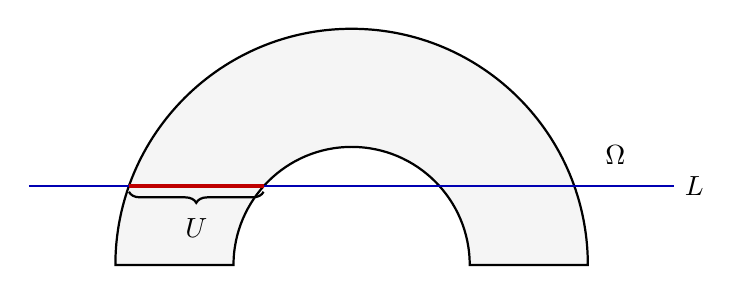
\begin{tikzpicture}[scale=1.0, line width=0.7pt]
  % Domain Omega: half-annulus (concave shape, so L can cut it into multiple components)
  \draw[thick, fill=black!4]
    (-3,0) arc[start angle=180, end angle=0, radius=3]
    -- (1.5,0) arc[start angle=0, end angle=180, radius=1.5]
    -- cycle;
  \node at (3.35,1.4) {$\Omega$};
  % Complex line L (drawn as a real line, per our convention)
  \draw[blue!70!black, thick] (-4.1,1) -- (4.1,1) node[right, black] {$L$};
  % U: left connected component of L \cap Omega
  \draw[red!75!black, line width=1.4pt] (-2.828,1) -- (-1.118,1);
  % Brace below the segment so the picture is also clear in black-and-white
  \draw[decorate, decoration={brace, mirror, amplitude=4pt, raise=2pt}, thick]
    (-2.828,1) -- (-1.118,1);
  \node[below=8pt] at (-1.973,1) {$U$};
\end{tikzpicture}
\caption{A domain $\Omega$ cut by a complex line $L$.}
\label{fig:psh}
\end{figure}

\begin{example}\label{ex:pshfunctions:L104}
    When $n=0$, we have a canonical bijection $\PSH(\Omega)\cong \mathbb{R}$.
\end{example}

\begin{example}
    When $n=1$, we have $\PSH(\Omega)=\SH(\Omega)$.
\end{example}

Similar to \cref{thm:sh_rigid}, we have a rigidity theorem for plurisubharmonic functions as well.
\begin{theorem}\label{thm:psh_rigid}
    Let $\varphi\colon \Omega\rightarrow [-\infty,\infty)$ be a measurable function. Then the following are equivalent:
    \begin{enumerate}
        \item\label{itm:thm:psh_rigid:1} $\varphi$ is locally integrable and $\ddc\varphi\geq 0$;
        \item\label{itm:thm:psh_rigid:2} $\varphi$ coincides almost everywhere with a plurisubharmonic function $\psi$ on $\Omega$.
    \end{enumerate}
    Moreover, the plurisubharmonic function $\psi$ is unique.
\end{theorem}
Here, the operator $\ddc$ is normalized so that
\[
\ddc =\frac{\mathrm{i}}{2\pi}\partial \overline{\partial}.
\]
For the proof, we refer to \cite[Proposition~1.43]{GZ17}.

Plurisubharmonic functions have nice functorialities:
\begin{proposition}\label{prop:func_domain}
    Let $n'\in \mathbb{N}$ and $\Omega'\subseteq \mathbb{C}^{n'}$ be a domain. Given any holomorphic map $f\colon \Omega\rightarrow \Omega'$ and any $\varphi\in \PSH(\Omega')$, exactly one of the following cases occurs:
    \begin{enumerate}
        \item\label{itm:prop:func_domain:1} $f^*\varphi\equiv -\infty$;
        \item\label{itm:prop:func_domain:2} $f^*\varphi\in \PSH(\Omega)$.
    \end{enumerate}
\end{proposition}
We refer to \cite[Proposition~1.44]{GZ17} for the proof\footnote{Recall that the statement of \cite[Proposition~1.44]{GZ17} is flawed. One has to reduce to the case where Case~\ref{itm:prop:func_domain:1} does not occur before following their proof.}.

For each $n\in \mathbb{N}$, $a\in \mathbb{C}^n$ and $r>0$, we write
\begin{equation}\label{eq:Bnar}
B_n(a,r)=\left\{ z\in \mathbb{C}^n: |z-a|<r \right\}.
\end{equation}
\begin{proposition}\label{prop:ballpshconvex}
    Let $\varphi\in \PSH(B_n(a,r_0))$ for some $r_0>0$. Then the function
    \[
    (-\infty,\log r_0)\rightarrow \mathbb{R},\quad \log r\mapsto \sup_{B_n(a,r)}\varphi
    \]
    is convex and increasing.
\end{proposition}
See \cite[Theorem~4.1.13]{Hor07} for the case $n>1$ and \cite[Corollary~2.4]{Bou17} for the general case.

\begin{proposition}\label{prop:subhimplyconv}
Let $a<b$ be two real numbers.
    Let $f\colon (a,b)\rightarrow [-\infty,\infty)$ be a function. Define
    \[
    g\colon \{z\in \mathbb{C}:a<\Real z<b\}\rightarrow [-\infty,\infty),\quad z\mapsto f(\Real z).
    \]
    Suppose that $g$ is subharmonic. Then $f$ is convex. In particular, $f$ takes real values only.
\end{proposition}

See \cite[Theorem~2.12]{HK76} for a more general result.

\subsection{The manifold case}
\label{subsec:psh_manifold}
Let $X$ be a complex manifold. In the whole book, complex manifolds are assumed to be paracompact, namely, all connected components have countable bases.


\begin{definition}\label{def:pshmfd}
    A \emph{plurisubharmonic function}\index{plurisubharmonic function} on $X$ is a function $\varphi\colon X\rightarrow [-\infty,\infty)$ such that for any $x\in X$, there exists an open neighborhood $U$ of $x$ in $X$, an integer $n\in \mathbb{N}$, a domain $\Omega\subseteq \mathbb{C}^n$ and a biholomorphic map $F\colon \Omega\rightarrow U$ such that $F^*(\varphi|_U)\in \PSH(\Omega)$.

    The set of plurisubharmonic functions on $X$ is denoted by $\PSH(X)$\index{$\PSH(X)$}.
\end{definition}

\begin{example}\label{ex:pshfunctions:L172}
    When $X$ is a domain in $\mathbb{C}^n$, the notions of plurisubharmonic functions in \cref{def:pshmfd} and in \cref{def:psh} coincide.
\end{example}

\begin{example}\label{ex:pshfunctions:L176}
    Write $\{X_i\}_{i\in I}$ for the set of connected components of $X$. Then we have a natural bijection
    \[
    \PSH(X) \cong \prod_{i\in I} \PSH(X_i).
    \]
    Here the product is in the category of sets.
    In particular, if $X=\varnothing$, then $\PSH(X)$ is a singleton.
\end{example}
This example allows us to reduce to the case of connected manifolds when studying general plurisubharmonic functions.

\begin{proposition}\label{prop:pullbackpsh}
    Let $Y$ be a complex manifold and $f\colon Y\rightarrow X$ be a holomorphic map. Then for any $\varphi\in \PSH(X)$, exactly one of the following cases occurs:
    \begin{enumerate}
        \item\label{itm:prop:pullbackpsh:1} $f^*\varphi$ is identically $-\infty$ on some connected component of $Y$;
        \item\label{itm:prop:pullbackpsh:2} $f^*\varphi\in \PSH(Y)$.
    \end{enumerate}
\end{proposition}
This proposition follows from \cref{prop:func_domain} applied separately on each connected component of $Y$.

\cref{thm:psh_rigid} implies immediately the general form of the rigidity theorem:
\begin{theorem}\label{thm:psh_rigid_gen}
    Let $\varphi\colon X\rightarrow [-\infty,\infty)$ be a measurable function. Then the following are equivalent:
    \begin{enumerate}
        \item\label{itm:thm:psh_rigid_gen:1} $\varphi$ is locally integrable and $\ddc \varphi\geq 0$;
        \item\label{itm:thm:psh_rigid_gen:2} $\varphi$ coincides almost everywhere with a plurisubharmonic function $\psi$ on $X$.
    \end{enumerate}
    Moreover, the plurisubharmonic function $\psi$ in \ref{itm:thm:psh_rigid_gen:2} is unique.
\end{theorem}


\begin{definition}\label{def:pluripolarsets}
    A subset $E\subseteq X$ is \emph{pluripolar}\index{set!pluripolar set} if for any $x\in X$, there is an open neighborhood $U$ of $x$ in $X$ and a function $\psi\in \PSH(U)$ such that
    \[
    \psi|_{E\cap U}\equiv -\infty.
    \]
    A subset $E\subseteq X$ is \emph{non-pluripolar}\index{set!non-pluripolar set} if $E$ is not pluripolar.

    A subset $F\subseteq X$ is \emph{co-pluripolar}\index{set!co-pluripolar set} if $X\setminus F$ is pluripolar.
\end{definition}
When $X$ has dimension $1$, a pluripolar set is called a \emph{polar set}. We say some property about objects on $X$ holds \emph{quasi-everywhere}\index{quasi-everywhere} if it holds outside a pluripolar set.


\begin{theorem}[Josefson's theorem]\label{thm:Josefson}\index{theorem!Josefson's theorem}
    Let $E\subseteq \mathbb{C}^n$ be a pluripolar set. Then there is $\varphi\in \PSH(\mathbb{C}^n)$ such that $\varphi|_E\equiv -\infty$.
\end{theorem}
See \cite[Corollary~4.41]{GZ17} for the proof of a more general result.

There is also a global version of Josefson's theorem:
\begin{theorem}\label{thm:gloJosefson}
    Assume that $X$ is a compact complex manifold and $E\subseteq X$ is a pluripolar set. Then there is a quasi-plurisubharmonic function $\varphi$ on $X$ with $\varphi|_E\equiv -\infty$.
\end{theorem}
For a proof, see \cite{Vu19}. The notion of quasi-plurisubharmonic functions will be recalled in \cref{def:qpsh} below.


\section{Properties of plurisubharmonic functions}
\label{sec:psh_properties}
In this section, we explore the basic properties of plurisubharmonic functions.

Let $X$ be a complex manifold.

\begin{proposition}\label{prop:pshlocLp}
    Let $\varphi\in \PSH(X)$. Then for any $p\geq 1$, $\varphi\in L^p_{\loc}(X)$.
\end{proposition}
See \cite[Theorem~1.46, Theorem~1.48]{GZ17}.\footnote{We remind the readers that the third displayed formula in the proof of \cite[Theorem~1.48]{GZ17} Step~2 is wrong. But this is irrelevant for our purpose.}

\begin{proposition}\label{prop:pshfunction_closedseq}
\leavevmode
\begin{enumerate}
    \item\label{itm:prop:pshfunction_closedseq:1} Assume that $(\varphi_i)_{i\in I}$ is a non-empty family in $\PSH(X)$ that is locally uniformly bounded from above. Then $\uscsup[i\in I] \varphi_i\in \PSH(X)$.
    \item\label{itm:prop:pshfunction_closedseq:2} Assume that $(\varphi_i)_{i\in I}$ is a decreasing net in $\PSH(X)$ such that $\varphi\coloneqq \inf_{i\in I}\varphi_i$ is not identically $-\infty$ on any connected component of $X$. Then $\varphi\in \PSH(X)$. Furthermore, $\varphi_i\xrightarrow{L^1_{\loc}} \varphi$.
\end{enumerate}
\end{proposition}
Here $\uscsup$ denotes the upper semicontinuous regularization of the supremum. When $I$ is a finite family, observe that
\[
\uscsup[i\in I]\varphi_i=  \sup_{i\in I}\varphi_i.
\]
When $I=\{1,\ldots,m\}$, we write
\[
    \varphi_1\lor \cdots\lor \varphi_m\coloneqq   \sup_{i\in I}\varphi_i.
\]
We refer to \cite[Proposition~1.28, Proposition~1.40]{GZ17}\footnote{In \cite[Proposition~1.28]{GZ17}, the second part is only stated for sequences, the net version is obvious using the sub-mean value inequality and the monotone convergence theorem for nets as in \cite[Proposition~7.12]{Fol99}.}\footnote{The proof of \cite[Proposition~1.40]{GZ17} contains a gap: The measurability of $u$ is not established during the proof, so the claim $u \ast \chi_{\epsilon}$ converges to $u$ in $L^1_{\loc}$ is not valid. One needs to choose the sequence $(v_j)_j$ carefully so that $v\leq u$, and use the fact that $v \ast \chi_{\epsilon}$ converges to $v$ in $L^1_{\loc}$ instead.}.

\begin{proposition}[Choquet's lemma]\label{prop:Choquet}\index{theorem!Choquet's lemma}
    Assume that $X$ has countably many connected components.
    Assume that $(\varphi_i)_{i\in I}$ is a non-empty family in $\PSH(X)$ that is locally uniformly bounded from above. There exists a countable subset $J\subseteq I$ such that
    \[
    \uscsup[i\in I] \varphi_i=\uscsup[j\in J] \varphi_j.
    \]
\end{proposition}
In the sequel, we say a subset $B\subseteq X$ is a \emph{holomorphic ball}\index{holomorphic ball} if $B$ has smooth boundary in $X$, and $B$ is biholomorphic to an open ball in $\mathbb{C}^n$.

\begin{proof}
    We may assume that $X$ is connected. Since by our convention, the complex manifold $X$ is paracompact, it can be covered by countably many holomorphic balls, so we can easily reduce to the case where $X$ is an open ball in $\mathbb{C}^n$. In this case, the result is proved in \cite[Lemma~4.31]{GZ17}.
\end{proof}



\begin{proposition}\label{prop:ppsnull}
    A pluripolar set $E\subseteq X$ is a Lebesgue null set.
\end{proposition}
\begin{proof}
    This is a trivial consequence of \cref{prop:pshlocLp}.
\end{proof}

\begin{proposition}\label{prop:supsupstardiff}
    Let $(\varphi_i)_{i\in I}$ be a non-empty family in $\PSH(X)$ that is locally uniformly bounded from above. Then the set
    \[
        \left\{x\in X: \sup_{i\in I}\varphi_i<\uscsup[i\in I]\varphi_i \right\}
    \]
    is pluripolar and hence Lebesgue null.
\end{proposition}
See \cite[Corollary~4.28]{GZ17}.




\begin{proposition}\label{prop:pshfuncdetdense}
    Suppose that $\varphi,\psi\in \PSH(X)$. If $\varphi\leq \psi$ almost everywhere, then $\varphi\leq \psi$ everywhere.

    In particular, if $\varphi=\psi$ almost everywhere, then $\varphi=\psi$ everywhere.
\end{proposition}
\begin{proof}
    Replace $\varphi$ by $\varphi\lor\psi$. Then $\varphi,\psi$ are two plurisubharmonic functions that coincide almost everywhere. The uniqueness statement in \cref{thm:psh_rigid_gen} gives $\varphi=\psi$.
\end{proof}


\begin{proposition}\label{prop:pluripolarunion}
    Let $(E_i)_{i\in \mathbb{Z}_{>0}}$ be a sequence of pluripolar sets in $X$. Then
    \[
    E\coloneqq \bigcup_{i=1}^{\infty}E_i
    \]
    is also pluripolar.
\end{proposition}
\begin{proof}
    The problem is local, so we may assume that $X\subseteq \mathbb{C}^n$ is a bounded domain. In this case, by \cref{thm:Josefson} for each $i\in \mathbb{Z}_{>0}$ we can choose $\psi_i\in \PSH(\mathbb{C}^n)$ such that
    \[
    \psi_i|_{E_i}\equiv -\infty,\quad \psi_i|_X\leq 0
    \]
    for all $i>0$. By \cref{prop:pshlocLp}, we have $\psi_i|_X\in L^1(X)$ for all $i>0$. After rescaling, we may also assume that $\|\psi_i\|_{L^1(X)}\leq 1$ for all $i>0$.

    We then define
    \[
    \psi=\sum_{i=1}^{\infty}2^{-i} \psi_i|_X.
    \]
    Then $\psi\in \PSH(X)$ according to \cref{prop:pshfunction_closedseq} and $\psi|_{E}=-\infty$.
\end{proof}



\begin{corollary}\label{cor:L1limipp}
    Let $(\varphi_j)_{j\in \mathbb{Z}_{>0}}$ be a sequence in $\PSH(X)$ such that $\varphi_j\xrightarrow{L^1_{\loc}}\varphi\in \PSH(X)$. Then
    \begin{equation}\label{eq:L1limsup1}
        \varphi=\mathop{\vphantom{\operatorname{sup}^{*}}\inf}\limits_{j>0} \uscsup[k\geq j]\varphi_k,
    \end{equation} and the set
    \[
        \left\{x\in X: \varphi(x)\neq \varlimsup_{j\to\infty}\varphi_j(x)\right\}
    \]
    is pluripolar.
\end{corollary}
\begin{proof}
    We may assume that $X$ is connected.

    We first observe that $(\varphi_j)_j$ is locally uniformly bounded from above. This follows from \cite[Exercise~1.20]{GZ17}.

    For each $j\geq 1$, let
    \[
        \psi_j=\uscsup[k\geq j]\varphi_k.
    \]
    Then $\psi_j\in \PSH(X)$ by \cref{prop:pshfunction_closedseq}. Moreover, $(\psi_j)_j$ is a decreasing sequence and $\psi_j\geq \varphi_j$ for all $j$.
    After considering a subsequence of $(\varphi_j)_j$ which converges to $\varphi$ almost everywhere, we get $\varphi\leq \psi\coloneqq \inf_j \psi_j$ almost everywhere. In particular, $\psi\in \PSH(X)$ by \cref{prop:pshfunction_closedseq}.

    On the other hand, by \cref{prop:supsupstardiff}, there exist pluripolar sets $Z_j\subseteq X$ such that
    \[
    \psi_j=\sup_{k\geq j}\varphi_k
    \]
    on $X\setminus Z_j$. Let
    \[
    Z=\bigcup_{j=1}^{\infty} Z_j.
    \]
    Then $Z$ is a pluripolar set by \cref{prop:pluripolarunion}, and for any $x\in X\setminus Z$, we have $\psi(x)=\varlimsup_j \varphi_j(x)$.
    Moreover, $\psi=\varphi$ almost everywhere by \cite[Theorem~1.46]{GZ17}, and hence everywhere by \cref{prop:pshfuncdetdense}. Hence we conclude \eqref{eq:L1limsup1}.
    Moreover, for all $x\in X\setminus Z$,
    \[
        \varphi(x)=\varlimsup_{j\to\infty}  \varphi_j(x).
    \]
    This completes the proof.
\end{proof}


\begin{theorem}[Brelot, Grauert--Remmert]\label{thm:GRexten}\index{theorem!Grauert--Remmert extension theorem}
    Let $Z$ be an analytic subset in $X$ and $\varphi\in \PSH(X\setminus Z)$. Then the function $\varphi$ admits an extension to $\PSH(X)$ in the following two cases:
    \begin{enumerate}
        \item\label{itm:thm:GRexten:1} The set $Z$ has codimension at least $2$ everywhere.
        \item\label{itm:thm:GRexten:2} The set $Z$ has codimension at least $1$ everywhere and $\varphi$ is locally bounded from above near each point of $Z$.
    \end{enumerate}
    In both cases, the extension is unique and is given by
    \begin{equation}\label{eq:GRextvarphiexp}
    \varphi(x)=\varlimsup_{X\setminus Z\ni y\to x}\varphi(y),\quad x\in Z.
    \end{equation}
\end{theorem}
\begin{figure}[ht]
\centering
\begin{tikzpicture}[scale=0.95, line width=0.6pt, every node/.style={font=\small}]
  \def\R{2.6}
  \def\Re{0.55}
  % 3D sphere: outline + equator (front solid, back dashed)
  \draw[thick] (0,0) circle (\R);
  \draw[thick]         (-\R,0) arc[start angle=180, end angle=360, x radius=\R, y radius=\Re];
  \draw[thick, dashed] (-\R,0) arc[start angle=180, end angle=  0, x radius=\R, y radius=\Re];
  % Boundary label
  \draw[-{Stealth[length=2.5mm]}, thin] (3.6,1.85) -- (1.95,1.7);
  \node[anchor=west, inner sep=2pt] at (3.6,1.85) {$\partial B_n(z,r)$};
  % Z: connected 1-dim curve through z; outside the ball solid, inside dashed
  % (suggesting it lives in the back hemisphere within the ball, so L_j drawn
  % in the front are disjoint from Z\cap B in 3D).
  \draw[thick] (-3.65, 2.05) .. controls (-3.0, 1.55) and (-2.75, 1.25) .. (-2.42, 0.95);
  \draw[thick, densely dashed]
    (-2.42, 0.95) .. controls (-1.5, 0.5) and (-0.6, 0.15) .. (0, 0)
    .. controls (0.6, -0.15) and (1.5, -0.5) .. (2.42, -0.95);
  \draw[thick] (2.42, -0.95) .. controls (2.75, -1.25) and (3.0, -1.55) .. (3.65, -2.05);
  \node at (3.85, -1.65) {$Z$};
  % Point z at the centre of the sphere
  \fill (0,0) circle (1.7pt);
  \node[anchor=north east, inner sep=2pt] at (0,0) {$z$};
  % Approximating lines L_j through x_j -- different (non-parallel) tilts.
  \draw[gray, thin] ($ (1.5, 0.9) + 3.0*(0.2924, 0.9563) $) --
                    ($ (1.5, 0.9) - 3.0*(0.2924, 0.9563) $);
  \fill (1.5, 0.9) circle (1.3pt) node[right=1pt, black] {$x_1$};
  \node[inner sep=2pt] at ($ (1.5,0.9)+2.55*(0.2924,0.9563) $) {$L_1$};
  \draw[gray, thin] ($ (0.9, 0.4) + 3.0*(0.0872, 0.9962) $) --
                    ($ (0.9, 0.4) - 3.0*(0.0872, 0.9962) $);
  \fill (0.9, 0.4) circle (1.3pt) node[right=1pt, black] {$x_2$};
  \node[inner sep=2pt] at ($ (0.9,0.4)+2.65*(0.0872,0.9962) $) {$L_2$};
  \draw[gray, thin] ($ (0.4, 0.15) + 3.0*(-0.0349, 0.9994) $) --
                    ($ (0.4, 0.15) - 3.0*(-0.0349, 0.9994) $);
  \fill (0.4, 0.15) circle (1.3pt) node[right=1pt, black] {$x_3$};
  \node[inner sep=2pt] at ($ (0.4,0.15)+2.75*(-0.0349,0.9994) $) {$L_3$};
  \draw[blue!70!black, line width=1pt] (0,-2.95) -- (0,2.95);
  \node[above, black, inner sep=2pt] at (-0.18, 2.95) {$L$};
  % U: open neighborhoods of L \cap \partial B
  \draw[red!75!black, thick, fill=red!10] (0, 2.60) circle (0.30);
  \draw[red!75!black, thick, fill=red!10] (0,-2.60) circle (0.30);
  \draw[-{Stealth[length=2.5mm]}, red!75!black, thin] (-1.4, 2.6) -- (-0.36, 2.6);
  \node[red!75!black, anchor=east, inner sep=2pt] at (-1.4, 2.6) {$U$};
  \draw[-{Stealth[length=2.5mm]}, red!75!black, thin] (-1.4,-2.6) -- (-0.36,-2.6);
  \node[red!75!black, anchor=east, inner sep=2pt] at (-1.4,-2.6) {$U$};
\end{tikzpicture}
\caption{Notation in the proof of \itemref{itm:thm:GRexten:1}.}
\label{fig:GR}
\end{figure}
\begin{proof}
    The extension is unique thanks to \cref{prop:pshfuncdetdense}. We shall prove the existence.

    \ref{itm:thm:GRexten:2} Thanks to the uniqueness of the extension, the problem is local, so we may assume that $X$ is a domain in $\mathbb{C}^n$ with $n>0$ and there is a non-zero holomorphic function $f$ on $X$ vanishing on $Z$. For each $\epsilon>0$, we claim that the function $\varphi_{\epsilon}$ defined by
    \[
    \varphi_{\epsilon}(x)\coloneqq \left\{
    \begin{aligned}
        \varphi(x)+\epsilon\log|f(x)|^2,&\quad x\in X\setminus Z;\\
        -\infty,&\quad x\in Z
    \end{aligned}
    \right.
    \]
    is plurisubharmonic on $X$. By \cref{def:psh}, it suffices to verify the case $n=1$. In this case, we may assume that $Z=\{0\}$.
    It is clear that $ \varphi_{\epsilon}\in \SH(X\setminus Z)$.
    It suffices to verify the sub-mean value inequality at $0$, which is immediate.

    Next observe that the net $\varphi_{\epsilon}$ is increasing as $\epsilon\searrow 0$ and $\varphi_{\epsilon}$ is locally uniformly bounded from above. It follows from \cref{prop:pshfunction_closedseq} that $\tilde{\varphi}\coloneqq \uscsup[\epsilon>0]\varphi_{\epsilon}\in \PSH(X)$. Moreover, $\tilde{\varphi}$ clearly extends $\varphi$. Note that \eqref{eq:GRextvarphiexp} follows from the construction.

    \ref{itm:thm:GRexten:1} We invite the reader to consult \cref{fig:GR} for the notations used in the proof.

    Thanks to \ref{itm:thm:GRexten:2}, it suffices to verify that $\varphi$ is locally bounded from above near each point of $Z$. The problem is local, so we may assume that $X$ is a domain in $\mathbb{C}^n$ with $n\geq 2$.

    Suppose the assertion fails. Then there exist $z\in Z$ and a sequence $(x_j)_{j\geq 1}$ in $X\setminus Z$ converging to $z$ such that
    \begin{equation}\label{eq:limphiinfty_temp1}
    \lim_{j\to\infty} \varphi(x_j)=\infty.
    \end{equation}
    Since $Z$ has codimension at least $2$\footnote{In fact, codimension at least~$1$ suffices for this step.}, we may choose a complex line $L$ through $z$ which meets $Z$ in a discrete set; after shrinking $X$ we may further assume that
    \[
        L\cap Z=\{z\}.
    \]
    Pick an open ball $B_n(z,r)\Subset X$. After adding a constant to $\varphi$, we may arrange $\varphi<0$ on $L\cap \partial B_n(z,r)$. Since $\varphi$ is upper semicontinuous, there is an open
    neighborhood $U\subseteq X\setminus Z$ of $L\cap \partial B_n(z,r)$ such that
    \[
        \varphi|_U<0.
    \]

    For each $j\geq 1$ we now choose a complex line $L_j$ through $x_j$, disjoint from $Z\cap B_n(z,r)$, with $L_j\to L$ as $j\to\infty$ (the convergence being in the Grassmannian of affine complex lines in $\mathbb{C}^n$). The existence of such $L_j$ is precisely where the assumption $\operatorname{codim} Z\geq 2$ enters: after replacing $B_n(z,r)$ by a slightly smaller ball if necessary, the closure of $Z\cap B_n(z,r)$ is analytic in a neighborhood of the closed ball. The projection to the space of directions is proper on this compact analytic set, so by Remmert's theorem its image is contained in a proper analytic subset of $\mathbb{P}^{n-1}$. Hence its complement contains directions arbitrarily close to that of $L$.

    For $j$ large enough we now have
    \[
        L_j\cap \partial B_n(z,r)\subseteq U,
    \]
    so applying the maximum principle to $\varphi|_{L_j\cap X}$ at $x_j$ yields $\varphi(x_j)<0$, contradicting \eqref{eq:limphiinfty_temp1}.
\end{proof}



\begin{lemma}\label{lma:invariantpshfunfinite}
    Let $\varphi\in \PSH((\Delta^*)^n)$ be an $(S^1)^n$-invariant plurisubharmonic function. Then $\varphi$ is finite everywhere.
\end{lemma}
Here
\[
\Delta^*\coloneqq \{z\in \mathbb{C}: 0<|z|<1\}
\]
denotes the punctured unit disk.
\begin{proof}
    It clearly suffices to handle the case $n=1$. In this case, by \cite[Theorem~2.12]{HK76}, the map
    \[
    \log r\mapsto \int_{0}^{1} \varphi\left(r\mathrm{e}^{2\pi\mathrm{i}\theta}\right)\,\mathrm{d}\theta=\varphi(r)
    \]
    is a convex function of $\log r$.
    So, the set $\{r\in (0,1): \varphi(r)=-\infty\}$ is convex.
    But $\varphi$ is almost everywhere finite by \cref{prop:pshlocLp}. Since $\varphi$ is $S^1$-invariant, $\varphi|_{(0,1)}$ is almost everywhere finite.
    It follows from the convexity that it is everywhere finite.
\end{proof}




\begin{proposition}[Kiselman's principle]\label{prop:Kis}\index{theorem!Kiselman's principle}
Let $\Omega\subseteq \mathbb{C}^m\times \mathbb{C}^n$ be a pseudoconvex domain. Assume that for each $z\in \mathbb{C}^m$, the set
\[
    \Omega_z\coloneqq \bigl\{w\in\mathbb{C}^n: (z,w)\in \Omega \bigr\}
\]
has the form $E+\mathrm{i}\mathbb{R}^n$, where $E\subseteq \mathbb{R}^n$ is a subset. Let $\varphi\in \PSH(\Omega)$, assume that $\varphi$ is independent of the imaginary part of the variable in $\mathbb{C}^n$. Let $\Omega'$ be the projection of $\Omega$ to $\mathbb{C}^m$. Define $\psi\colon \Omega'\rightarrow [-\infty,\infty)$ as follows:
\[
    \psi(z)=\inf_{w\in \Omega_z}\varphi(z,w).
\]
Then either $\psi\equiv -\infty$ or $\psi\in \PSH(\Omega')$.
\end{proposition}
See \cite[Theorem~7.5]{DemBook} for the proof as well as the notion of pseudoconvex domains.

\begin{lemma}\label{lma:gl}
    Let $\Omega\subseteq \mathbb{C}^n$ be a domain and $\Omega'\subseteq \Omega$ be a subdomain. Consider $\varphi\in \PSH(\Omega)$ and $\psi\in \PSH(\Omega')$. Assume that
    \begin{equation}\label{eq:gluecond}
    \varliminf_{\substack{\Omega'\ni y\to x,\\ \psi(y)\neq -\infty}}\bigl(\varphi(y)-\psi(y)\bigr)\geq 0
    \end{equation}
    for any $x\in \Omega\cap \partial \Omega'$. Define
    \[
    \eta(z)=\left\{
    \begin{aligned}
        \varphi(z)\lor \psi(z),&\quad \text{if }z\in \Omega',\\
        \varphi(z),&\quad \text{if }z\in \Omega\setminus\Omega'.
    \end{aligned}
    \right.
    \]
    Then $\eta\in \PSH(\Omega)$.
\end{lemma}
This is essentially \cite[Proposition~1.30]{GZ17}. Since the statement in the reference is slightly misleading for our purposes, we include the proof for clarification.
\begin{figure}[ht]
\centering
\begin{tikzpicture}[scale=0.85, line width=0.6pt]
  % Omega: ellipse (so the boundary points are computable)
  \draw[thick, fill=black!4] (0,0) ellipse[x radius=4.0, y radius=2.5];
  \node at (4.4,2.0) {$\Omega$};
  % Dividing curve  partial Omega' \cap Omega. Endpoints are exactly on the
  % ellipse, and the midpoint at t=0.5 is the point (0.7, 0).
  \draw[thick] (1.000, 2.421)
    .. controls (1.000, 0.800) and (0.400, -0.776) .. (0.400, -2.487);
  \node at (-2.6, 0.0) {$\Omega'$};
  % Hatched region  U_x \cap Omega'  (left part of U_x, clipped to disc)
  \begin{scope}
    \clip (0.7, 0) circle (0.85);
    \fill[pattern=north east lines, pattern color=red!50] (-1, -1) rectangle (0.7, 1);
  \end{scope}
  % U_x disc
  \draw[red!75!black, thick] (0.7, 0) circle (0.85);
  % U_x label moved to upper-right, away from the dividing curve
  \node[red!75!black, anchor=west, inner sep=2pt] at (1.7, 1.05) {$U_x$};
  \draw[red!75!black, thin] (1.7, 1.05) -- (1.30, 0.50);
  % U_x \cap Omega' label moved to lower-left, away from the dividing curve
  \node[red!75!black, anchor=east, inner sep=2pt] at (-0.6, -1.05) {$U_x\cap\Omega'$};
  \draw[red!75!black, thin] (-0.6, -1.05) -- (-0.05, -0.55);
  % Point x exactly on the dividing curve
  \fill (0.7, 0) circle (1.6pt);
  \node[anchor=west, inner sep=2pt] at (0.78, 0) {$x$};
  % Point y inside  U_x \cap Omega' -- black dot + leader arrow + label outside
  \fill (0.25, 0.40) circle (1.6pt);
  \draw[-{Stealth[length=2mm]}, thin] (-0.55, 1.45) -- (0.20, 0.50);
  \node[anchor=east, inner sep=2pt] at (-0.55, 1.45) {$y$};
\end{tikzpicture}
\caption{Gluing procedure}
\label{fig:glue}
\end{figure}
\begin{proof}
See \cref{fig:glue} for the notations used in the proof.

    Take $\epsilon>0$.
    We first define
    \[
    \eta_{\epsilon}(z)=\begin{cases}
        \varphi(z)\lor (\psi(z)-2\epsilon),& \textup{if }z\in \Omega';\\
        \varphi(z),& \textup{if }z\in \Omega\setminus\Omega'.
    \end{cases}
    \]
    We claim that
    \[
    \eta_{\epsilon}\in \PSH(\Omega).
    \]
    By our assumption, for each $x\in \Omega\cap \partial \Omega'$, we can find an open neighborhood $U_x\subseteq \Omega$ such that for any $y\in U_x\cap \Omega'$, we have $\varphi(y)\geq \psi(y)-\epsilon$.
    Therefore, by taking a union of the $U_x$'s for various $x$, there is an open neighborhood $U$ of $\Omega\cap \partial \Omega'$ such that
    \[
    \varphi(y)\geq \psi(y)-\epsilon,\quad \forall y\in U\cap \Omega'.
    \]
    Since $U$ contains $\Omega\cap\partial\Omega'$, the set $(\Omega\setminus \Omega')\cup U$ is open in $\Omega$. On this open set we have $\eta_{\epsilon}=\varphi$, hence $\eta_{\epsilon}$ is plurisubharmonic there. It is plurisubharmonic on $\Omega'$ by \cref{prop:pshfunction_closedseq}. These two descriptions agree on the overlap $U\cap\Omega'$, so our claim follows from the local nature of plurisubharmonicity.

    Next we observe that as $\epsilon$ decreases to $0$, the functions $\eta_{\epsilon}$ increase to $\eta$. The family $(\eta_\epsilon)_{0<\epsilon\leq 1}$ is locally uniformly bounded from above. This is clear away from $\Omega\cap\partial\Omega'$. Near $\Omega\cap\partial\Omega'$, applying the previous estimate with $\epsilon=1$ gives an open neighborhood $U_1$ of $\Omega\cap\partial\Omega'$ such that $\psi\leq \varphi+1$ on $U_1\cap\Omega'$, hence $\eta_\epsilon\leq \varphi+1$ on $U_1$ for all $0<\epsilon\leq 1$. Therefore, $\eta^*\in \PSH(\Omega)$ by \cref{prop:pshfunction_closedseq}.

    It remains to observe that $\eta$ is upper semicontinuous. This is only non-trivial on the boundary of $\Omega'$. Take $x\in \Omega\cap \partial \Omega'$ and let $(y_i)_{i>0}$ be a sequence in $\Omega'$ with limit $x$. We first show that
    \begin{equation}\label{eq:limsuppsiphitemp1}
    \varlimsup_{i\to\infty} \psi(y_i)\leq \varphi(x).
    \end{equation}
    We may assume that $\psi(y_i)\neq -\infty$ for all $i>0$ and the left-hand side of \eqref{eq:limsuppsiphitemp1} is not $-\infty$. Then we can compute
    \[
    \varlimsup_{i\to\infty} \psi(y_i)\leq \varlimsup_{i\to\infty} \psi(y_i)+\varliminf_{i\to\infty} \bigl(\varphi(y_i)-\psi(y_i)\bigr)\leq \varlimsup_{i\to\infty}\varphi(y_i)\leq \varphi(x).
    \]
    Combining this with the upper semicontinuity of $\varphi$, we get
    \[
        \varlimsup_{i\to\infty}\bigl(\varphi(y_i)\lor\psi(y_i)\bigr)\leq \varphi(x)=\eta(x).
    \]
    This proves upper semicontinuity across $\Omega\cap\partial\Omega'$.
    Therefore, $\eta=\eta^*\in \PSH(\Omega)$.
\end{proof}

Note that the boundary condition \eqref{eq:gluecond} enters the proof only through \eqref{eq:limsuppsiphitemp1}, therefore, we can formulate a variant of \cref{lma:gl}:
\begin{corollary}\label{cor:glbdry}
    Let $\Omega\subseteq \mathbb{C}^n$ be a domain and $\Omega'\subseteq \Omega$ be a subdomain\footnote{In \cite[Proposition~1.30]{GZ17}, Guedj--Zeriahi assumed in addition that $\Omega'$ is relatively compact in $\Omega$. This assumption is not necessary for the proof, and the applications of this proposition in \cite{GZ17} usually do not satisfy this condition.}. Consider $\varphi\in \PSH(\Omega)$ and $\psi\in \PSH(\Omega')$. Assume that
    \[
        \varlimsup_{\Omega'\ni y\to x}\psi(y)\leq \varphi(x)
    \]
    for any $x\in \Omega\cap\partial\Omega'$. Define
    \[
    \eta(z)=\begin{cases}
        \varphi(z)\lor \psi(z),&\quad \textup{if }z\in \Omega';\\
        \varphi(z),&\quad \textup{if }z\in \Omega\setminus\Omega'.
    \end{cases}
    \]
    Then $\eta\in \PSH(\Omega)$.
\end{corollary}


Using the ideas of \cref{lma:gl} and the solution of the homogeneous Monge--Ampère equations on a strong pseudoconvex domain, one can prove the following:
\begin{proposition}\label{prop:BT_balayage}
Let $\Omega \subseteq \mathbb{C}^n$ be a domain, let $D \Subset \Omega$ be a strongly pseudoconvex domain, and let $\varphi \in \PSH(\Omega)$ be locally bounded.
Then there exists a unique locally bounded $\psi\in \PSH(\Omega)$
such that
\[
\begin{cases}
\left(\ddc\psi\right)^n = 0& \textup{on } D,\\
\psi = \varphi & \textup{on } \Omega\setminus D.
\end{cases}
\]
Moreover, $\psi\geq \varphi$.
\end{proposition}
See \cite[Proposition~9.1]{BT82} for the proof. We sometimes say $\psi$ is the \emph{balayage}\index{balayage} of $\varphi$ on $D$.

Let us also recall the following domination principle:
\begin{proposition}\label{prop:dom_prin_loc}
    Let $\Omega\subseteq \mathbb{C}^n$ be a bounded domain.
    Let $\varphi,\psi\in \PSH(\Omega)$ be locally bounded. Assume that
    \begin{enumerate}
        \item\label{itm:prop:dom_prin_loc:1} for each $z\in \partial \Omega$, we have
            \[
                \varliminf_{\Omega\ni w\to z} \Bigl(\psi(w)-\varphi(w)\Bigr)\geq 0;
            \]
        \item\label{itm:prop:dom_prin_loc:2} $\varphi\leq \psi$ a.e.\ with respect to $(\ddc \psi)^n$,
    \end{enumerate}
    Then $\varphi\leq \psi$.
\end{proposition}
This is \cite[Corollary~3.31]{GZ17}.\footnote{The statement in the reference is flawed, but the proof is correct.}

\section{Plurifine topology}\label{sec:plurifine}

In this section, we introduce the notion of plurifine topology. Unlike other sections in this chapter, this section contains full details. This is mainly due to the unfortunate omissions and numerous minor problems in the foundational paper \cite{BT87}. In particular, the key theorem \cref{thm:pf_basis} was claimed by Bedford--Taylor without proof. Our presentation largely follows \cite{EMW06}. We also include enough details so that this section is readable for those who are not familiar with the classical potential theory.

Very recently, El Kadiri--Fuglede published a book \cite{EKF} about classical fine potential theory, containing essentially all results in this section. The interested reader may consult their book for further details.

\subsection{Plurifine topology on domains}
\label{subsec:plurifine}
Let $\Omega\subseteq \mathbb{C}^n$ ($n\in \mathbb{N}$) be a domain.

\begin{definition}\label{def:pftopologydomain}
  The \emph{plurifine topology}\index{plurifine topology} on $\Omega$ is the weakest topology making all $\mathbb{R}$-valued plurisubharmonic functions on $\Omega$ continuous.
\end{definition}
We want to distinguish the Euclidean topology from the plurifine topology.
In the whole book, topological notions without adjectives refer to those with respect to the Euclidean topology. We include the symbol $\mathcal{F}$ in order to denote those with respect to the plurifine topology. For example, we will say $\mathcal{F}$-open subset, $\mathcal{F}$-neighborhood, $\mathcal{F}$-closure, etc.
The $\mathcal{F}$-closure of a set $E\subseteq \Omega$ will be denoted by $\overline{E}^{\mathcal{F}}$.

Recall that in the whole book, we follow Bourbaki's convention: a neighborhood is not necessarily open. Similarly, an $\mathcal{F}$-neighborhood is not necessarily $\mathcal{F}$-open.

A priori, we should include $\Omega$ into the notations as well, but as we will see shortly in \cref{cor:pf_compatible}, this is usually unnecessary.

When $n=0$, the domain $\Omega$ is a singleton and all assertions in this subsection are trivial. In the proofs below we therefore assume $n>0$.


\begin{proposition}\label{prop:pf_finer}
  The plurifine topology on $\Omega$ is finer than the Euclidean topology.
\end{proposition}
\begin{proof}
  It suffices to show that the unit ball $\{z\in \mathbb{C}^n:|z|<1\}$ is $\mathcal{F}$-open. This follows from the observation that this set can be written as
  \[
      \{\psi<0\} \quad\textup{with}\quad \psi(z)\coloneqq (\log |z|) \lor (-1).
  \]
  This completes the proof.
\end{proof}

\begin{example}\label{ex:pfopenpsh}
    Let $\varphi\in \PSH(\Omega)$ and $C\in \mathbb{R}$. Then the sets $\{\varphi>C\}$ and $\{\varphi<C\}$ are both $\mathcal{F}$-open.

    In fact, the latter case follows from \cref{prop:pf_finer}, while the former follows from the observation
    \[
    \{\varphi>C\}=\{\varphi\lor (C-1)>C\}.
    \]
\end{example}

\begin{definition}\label{def:pshfunctions:L691}
  A subset $E\subseteq \Omega$ is \emph{thin}\index{thin subset}\footnote{A more proper name would be \emph{plurithin}. But since we will never need the classical notion of thin sets à la Cartan in this book, we prefer omitting the prefix \emph{pluri-}.} at $x\in \Omega$ if one of the following conditions holds:
  \begin{enumerate}
    \item\label{itm:chapter-pshfunctions:L698:1} $x\not\in \overline{E}$;
    \item\label{itm:chapter-pshfunctions:L698:2} $x\in \overline{E}$ and there is an open neighborhood $U\subseteq \Omega$ of $x$ and $\varphi\in \PSH(U)$ such that
    \[
      \varlimsup_{(U\cap E)\setminus\{x\} \ni y\to x} \varphi(y)<\varphi(x).
    \]
  \end{enumerate}
  We say $E$ is \emph{thin} if it is thin at all $x\in \Omega$.
\end{definition}
\begin{remark}\label{rmk:cstthindef}
    In the second case, we can always arrange that
    \[
    \varphi|_{(E\setminus \{x\})\cap U}=0.
    \]
    In fact, we may assume that $\varphi\leq 0$ and $C<0$ is such that
    \[
    \varlimsup_{(U\cap E)\setminus\{x\} \ni y\to x} \varphi(y)<C<\varphi(x).
    \]
    We let
    \[
        \psi=(-C)^{-1}(\varphi\lor C)+1.
    \]
    Then $\psi$ satisfies our requirements for a smaller $U$.
\end{remark}

In the second case, the function $\varphi$ can be very much improved.
\begin{proposition}[Bedford--Taylor]\label{prop:BTthin}\index{theorem!Bedford--Taylor base theorem}
  Consider a set $E\subseteq \Omega$ and $x\in \overline{E}$. Assume that $E$ is thin at $x$. Then there is $\varphi\in \PSH(\mathbb{C}^n)$ with the following properties:
  \begin{enumerate}
    \item\label{itm:prop:BTthin:1} $\varphi$ is locally bounded outside $x$;
    \item\label{itm:prop:BTthin:2} $\varphi(x)>-\infty$;
    \item\label{itm:prop:BTthin:3}
    \[
    \lim_{E\setminus\{x\} \ni y\to x} \varphi(y)=-\infty.
    \]
  \end{enumerate}
\end{proposition}
\begin{proof}\footnote{The original argument in \cite[Proposition~10.2]{BT82} was quite intriguing: Neither the auxiliary functions $\varphi_j$'s nor the simple computations were correct. However, I believe that Bedford--Taylor had a correct proof in mind. Something more than a typo, but not yet a mistake, could be properly called a \emph{thinkpo}, a terminology invented by R.~Berman.}
By \cref{rmk:cstthindef}, there is an open neighborhood $U\subseteq \Omega$ of $x$ and $\psi\in \PSH(U)$ such that
\[
    \psi|_{U\cap (E\setminus\{x\})}=-1 \quad\textup{and}\quad \psi(x)=0.
\]
Without loss of generality we may assume $x=0$ and that $U=B_n(0,1)$ is the open unit ball.

Since $\psi$ is upper semicontinuous at $0$ with $\psi(0)=0$, we may choose a strictly decreasing sequence $(\delta_j)_{j\geq 1}\subseteq (0,\mathrm{e}^{-1})$ such that
\begin{equation}\label{eq:BTthin_choosedelta}
    \psi(y)<2^{-j-2}\quad\textup{whenever } |y|<\delta_j.
\end{equation}
In particular $|\log\delta_j|>1$ for every $j\geq 1$, so the series of constants
\begin{equation}\label{eq:BTthin_summable}
    \sum_{j=1}^\infty \frac{2^{-j-1}}{|\log\delta_j|} \leq \sum_{j=1}^\infty 2^{-j-1}=\frac{1}{2}
\end{equation}
converges. We further set
\[
    \gamma_j\coloneqq \exp\bigl(2^{j+1}\log\delta_j\bigr)=\delta_j^{2^{j+1}}\in(0,1),
\]
which is also decreasing in $j$.

For each $j\geq 1$ define
\[
    \varphi_j(z)\coloneqq
    \begin{cases}
        \frac{2^{-j-1}}{|\log\delta_j|}\log|z|\lor\bigl(\psi(z)-2^{-j}\bigr), &\textup{if } |z|<\delta_j,\\
        \frac{2^{-j-1}}{|\log\delta_j|}\log|z|,&\textup{if } |z|\geq \delta_j.
    \end{cases}
\]
On the boundary $|z|=\delta_j$, the logarithmic term tends to $-2^{-j-1}$. By \eqref{eq:BTthin_choosedelta},
\[
    \varlimsup_{|z|<\delta_j,\ z\to z_0}(\psi(z)-2^{-j})\leq 2^{-j-2}-2^{-j}<-2^{-j-1}
\]
for every $z_0$ with $|z_0|=\delta_j$. Hence the boundary condition in \cref{lma:gl} is satisfied. We obtain that $\varphi_j\in \PSH(\mathbb{C}^n)$.

By construction, $\varphi_j\leq 0$ on $U$, $\varphi_j(0)=-2^{-j}$, and for $z\in E\setminus\{0\}$ with $|z|<\gamma_j$ we have $\varphi_j(z)\leq -1$, since
\[
    \frac{2^{-j-1}}{|\log\delta_j|}\log|z|<\frac{2^{-j-1}}{|\log\delta_j|}\,(2^{j+1}\log\delta_j)=-1
\]
and, on $E\setminus\{0\}$, $\psi(z)-2^{-j}=-1-2^{-j}<-1$.

We then define
\[
    \varphi\coloneqq \sum_{j=1}^{\infty}\varphi_j.
\]
On the unit ball $U$ each $\varphi_j\leq 0$, so the partial sums $S_N\coloneqq \sum_{j=1}^N\varphi_j$ form a decreasing sequence of plurisubharmonic functions with
\[
    S_N(0)=-\sum_{j=1}^N 2^{-j}\to -1>-\infty,\quad \textup{as } N\to\infty
\]
so $\varphi|_U\in \PSH(U)$ by \cref{prop:pshfunction_closedseq}. On $\mathbb{C}^n\setminus B_n(0,\delta_1)$ each $\varphi_j$ equals $\frac{2^{-j-1}}{|\log\delta_j|}\log|z|$, and \eqref{eq:BTthin_summable} shows $S_N$ converges uniformly on every compact subset to $\bigl(\sum_{j\geq 1}\tfrac{2^{-j-1}}{|\log\delta_j|}\bigr)\log|z|$, a plurisubharmonic limit. Both formulas agree on $U\setminus B_n(0,\delta_1)$, so altogether $\varphi\in \PSH(\mathbb{C}^n)$.

We now verify the three claims.

  \emph{Property \ref{itm:prop:BTthin:2}}. This is the equality $\varphi(0)=-\sum_{j\geq 1}2^{-j}=-1>-\infty$ obtained above.

  \emph{Property \ref{itm:prop:BTthin:3}}. Fix $j_0\geq 1$. For $z\in E\setminus\{0\}$ with $|z|<\gamma_{j_0}$, the bound $\varphi_j(z)\leq -1$ holds for every
  $j\leq j_0$ (since the $\gamma_j$ are decreasing), while $\varphi_j(z)\leq 0$ for $j>j_0$. Hence $\varphi(z)\leq -j_0$, and
  letting $j_0\to \infty$ yields
  \[
    \varlimsup_{E\setminus \{0\} \ni y\to 0}\varphi(y)=-\infty.
  \]

  \emph{Property \ref{itm:prop:BTthin:1}.} Fix any $z_0\in \mathbb{C}^n$ with $z_0\neq 0$ and choose $J\geq 1$ such that $\delta_J<|z_0|/2$. On the open set
  $W=\{w\in \mathbb{C}^n:|w|>|z_0|/2\}$, all $\varphi_j$ with $j\geq J$ lie in the outer regime, and \eqref{eq:BTthin_summable} shows $\sum_{j\geq J}\varphi_j(w)
   =\bigl(\sum_{j\geq J}\tfrac{2^{-j-1}}{|\log\delta_j|}\bigr)\log|w|$ is locally bounded on $W$. The remaining finitely many terms $\varphi_1,\ldots,\varphi_{J-1}$ are plurisubharmonic on $\mathbb{C}^n$, hence locally bounded above on $W$, while $\varphi_j(w)\geq \tfrac{2^{-j-1}}{|\log\delta_j|}\log|w|$ keeps
  them locally bounded below as well. Therefore $\varphi$ is locally bounded on $W$. Since $z_0\neq 0$ was arbitrary, $\varphi$ is locally bounded on $\mathbb{C}^n\setminus\{0\}$, which is property~\ref{itm:prop:BTthin:1}.
\end{proof}

\begin{lemma}\label{lma:unionthin}
    Let $E_1,E_2\subseteq \Omega$. Assume that $E_1$, $E_2$ are both thin at $x\in \Omega$. Then so is $E_1\cup E_2$.
\end{lemma}
\begin{proof}
    We may assume that $x\in \overline{E_1}\cap \overline{E_2}$. Take an open neighborhood $U\subseteq \Omega$ of $x$ and $\varphi_1,\varphi_2\in \PSH(U)$ such that
    \[
        \varlimsup_{y\to x,y\in E_i\setminus\{x\}} \varphi_i(y)<\varphi_i(x),\quad i=1,2.
    \]
    Then $\varphi_1+\varphi_2\in \PSH(U)$ and
    \[
    \varlimsup_{y\to x,y\in (E_1\cup E_2)\setminus\{x\}} (\varphi_1+\varphi_2)(y)<\varphi_1(x)+\varphi_2(x).
    \]
    In particular, $E_1\cup E_2$ is thin at $x$.
\end{proof}

\begin{theorem}[H.~Cartan]\label{thm:Cartan}\index{theorem!H.~Cartan's coherence theorem}
  Consider a set $E\subseteq \Omega$ and $x\in E$.
  Then the following are equivalent:
  \begin{enumerate}
    \item\label{itm:thm:Cartan:1} $E$ is an $\mathcal{F}$-neighborhood of $x$;
    \item\label{itm:thm:Cartan:2} $\Omega\setminus E$ is thin at $x$.
  \end{enumerate}
\end{theorem}
\begin{proof}
  \ref{itm:thm:Cartan:2} $\implies$ \ref{itm:thm:Cartan:1}. Assume \ref{itm:thm:Cartan:2}. We may assume that $x\in \overline{\Omega\setminus E}$. Otherwise, our assertion follows from \cref{prop:pf_finer}.

  By \cref{prop:BTthin}, there is an open neighborhood $U$ of $x$ in $\Omega$ and $\varphi\in \PSH(\mathbb{C}^n)$ such that
  \[
      \varphi(x)>\sup_{y\in U\cap (\Omega\setminus E)} \varphi(y)\eqqcolon \lambda.
  \]
  Let $F=\{y\in \Omega: \varphi(y)>\lambda\}$. Then $x\in F$ and $F$ is $\mathcal{F}$-open by \cref{ex:pfopenpsh}. Moreover, $U\cap F\subseteq E$. By \cref{prop:pf_finer}, we conclude \ref{itm:thm:Cartan:1}.

  \ref{itm:thm:Cartan:1} $\implies$ \ref{itm:thm:Cartan:2}. Assume \ref{itm:thm:Cartan:1}. We may always replace $E$ by smaller $\mathcal{F}$-neighborhoods of $x$. In particular, we may assume that $E$ has the following form
  \[
      \{y\in U:\varphi_1(y)>\lambda_1,\ldots,\varphi_m(y)>\lambda_m\},
  \]
  where $U\subseteq \Omega$ is an open neighborhood of $x$, and $\varphi_1,\ldots,\varphi_m$ are $\mathbb{R}$-valued psh functions on $\Omega$, and $\lambda_1,\ldots,\lambda_m\in \mathbb{R}$. Since $x\in U$, the set $\Omega\setminus U$ is thin at $x$. Moreover,
    \[
        \Omega\setminus E=(\Omega\setminus U)\cup \bigcup_{i=1}^m\{y\in U:\varphi_i(y)\leq\lambda_i\}.
    \]
    By \cref{lma:unionthin}, it is enough to prove that each set $\{y\in U:\varphi_i(y)\leq\lambda_i\}$ is thin at $x$. Thus we may assume $m=1$. In this case, $\Omega\setminus E$ is clearly thin at $x$.
\end{proof}


\begin{theorem}\label{thm:pf_basis}
  A base of the plurifine topology on $\Omega$ is given by sets of the following form:
  \begin{equation}\label{eq:basis_fine}
    \left\{x\in U: \varphi(x)>0\right\},
  \end{equation}
  where $U\subseteq \Omega$ is an open subset and $\varphi\in \PSH(U)$.
\end{theorem}

\begin{proof}
  Observe that sets of the form \eqref{eq:basis_fine} are $\mathcal{F}$-open.\footnote{This is not entirely obvious by definition, as $\varphi$ is not defined on the whole $\Omega$.} By \cref{thm:Cartan}, it suffices to show its complement in $\Omega$ is thin at each point of \eqref{eq:basis_fine}, which is obvious.

  Now consider $x\in \Omega$ and an $\mathcal{F}$-open neighborhood $V\subseteq \Omega$ of $x$. We want to find a set of the form \eqref{eq:basis_fine} contained in $V$ and containing $x$.

  Write $E=\Omega\setminus V$. In case $x\in \Int V$, there is nothing to prove. So we may assume that $x\in \overline{E}$. By \cref{thm:Cartan}, $E$ is thin at $x$. By definition, there is an open neighborhood $U\subseteq \Omega$ of $x$ and $\varphi\in \PSH(U)$ such that
  \[
    \varlimsup_{y\to x,y\in U\cap (E\setminus\{x\})}\varphi(y)<\varphi(x).
  \]
  We may assume that $\varphi|_{E\cap U}\leq 0<\varphi(x)$. Then the set $\{y\in U:\varphi(y)>0\}$ suffices for our purpose.
\end{proof}

\begin{remark}
    Recall that in general, an $\mathcal{F}$-open set is \emph{not} a \emph{countable} union of sets of the form \eqref{eq:basis_fine}. In fact, an $\mathcal{F}$-open set is not a Borel set in general.
    See \cite{EK23} for a concrete example.
\end{remark}

\begin{corollary}\label{cor:pf_compatible}
  Let $\Omega_1\subseteq \Omega_2\subseteq \mathbb{C}^n$ be two non-empty open subsets. Then the plurifine topology on $\Omega_1$ is the same as the subspace topology induced from the plurifine topology on $\Omega_2$.
\end{corollary}
In particular, when we talk about an $\mathcal{F}$-open set $U$ in $\mathbb{C}^n$, we no longer have to specify the domain $\Omega\supseteq U$.

\begin{corollary}\label{cor:compactnhformbase}
  Let $\Omega\subseteq \mathbb{C}^n$ be an $\mathcal{F}$-open subset and $x\in \Omega$. Then $x$ has a compact $\mathcal{F}$-neighborhood contained in $\Omega$.
\end{corollary}
\begin{proof}
  By \cref{thm:pf_basis}, it suffices to prove the assertion after replacing $\Omega$ by a smaller $\mathcal F$-open neighborhood of $x$. Thus we may assume that
    \[
        \Omega=\{y\in U:\varphi(y)>0\}
    \]
    for some open set $U\subseteq\mathbb C^n$ and some $\varphi\in\PSH(U)$.

  Take a compact neighborhood $K$ of $x$ in $U$. Now $\{y\in K: \varphi(y)\geq \varphi(x)/2\}$ is a compact $\mathcal{F}$-neighborhood of $x$ contained in $\Omega$.
\end{proof}

\begin{corollary}\label{cor:holomappfcont}
    Let $\Omega\subseteq \mathbb{C}^n$, $\Omega'\subseteq \mathbb{C}^{n'}$ be two domains and $F\colon \Omega'\rightarrow \Omega$ be a holomorphic map. Then $F$ is $\mathcal{F}$-continuous.
\end{corollary}

\begin{proof}
    It suffices to show that the inverse image $F^{-1}(U)$ of each $\mathcal{F}$-open subset $U\subseteq \Omega$ is $\mathcal{F}$-open.
    By \cref{thm:pf_basis}, after possibly shrinking $\Omega$ and $\Omega'$, we may assume that $U$ has the form $\{x\in \Omega:\psi(x)>0\}$, where $\psi \in \PSH(\Omega)$. Clearly, we may assume that $F^{-1}(U)$ is non-empty. Then $F^*\psi\in \PSH(\Omega')$ by \cref{prop:pullbackpsh}, we find that
    \[
        F^{-1}(U)=\{y\in \Omega': F^*\psi(y)>0\}
    \]
    is $\mathcal{F}$-open.
\end{proof}


\subsection{Plurifine topology on manifolds}\label{subsec:pftmfd}
Let $X$ be a complex manifold.
\begin{definition}\label{def:pftopologygeneral}
    The \emph{plurifine topology}\index{plurifine topology} on $X$ is the topology with a base consisting of sets of the form $F^{-1}(V)$, where $U\subseteq X$ is an open subset, $F\colon U\rightarrow \Omega$ is a biholomorphic map, $\Omega\subseteq \mathbb{C}^n$ is a domain for some $n\in \mathbb{N}$, and $V\subseteq \Omega$ is $\mathcal{F}$-open.
\end{definition}
Note that these sets form a topological base thanks to \cref{cor:holomappfcont}. Moreover, it also follows from \cref{cor:holomappfcont} that the plurifine topologies on domains defined in \cref{def:pftopologygeneral} and in \cref{def:pftopologydomain} coincide.

We refer to \cref{def:qpsh} for the notion of quasi-plurisubharmonic functions.
\begin{proposition}\label{prop:pshfunFcont}
    Let $\varphi\in \QPSH(X)$. Then $\varphi$ is $\mathcal{F}$-continuous.
\end{proposition}
\begin{proof}
    It suffices to show that $\varphi|_{\{\varphi\neq -\infty\}}$ is $\mathcal{F}$-continuous, since $\{\varphi=-\infty\}$ is $\mathcal{F}$-closed.

    The problem is local, so we may assume that $X\subseteq \mathbb{C}^n$ is a domain and $\varphi=\psi+g$, where $\psi\in \PSH(X)$ and $g\in C^{\infty}(X)$ and $|g|\leq C$ for some $C>0$. For an open interval $(a,b)\subseteq \mathbb{R}$, it suffices to show that
    \[
        U\coloneqq \left\{ x\in X:a<\varphi(x)<b\right\}=\left\{ x\in X:a-g(x)<\psi(x)<b-g(x)\right\}
    \]
    is $\mathcal{F}$-open. Take $x\in U$. We can find an open neighborhood $V$ of $x$ in $U$ such that
    \[
    \sup_{y\in V} \left( a-g(y)\right)<\psi(x)< \inf_{y\in V} \left( b-g(y) \right).
    \]
    Therefore,
    \[
    \left\{z\in V:\sup_{y\in V} \left(a-g(y)\right)<\psi(z)<\inf_{y\in V} \left(b-g(y)\right)\right\}
    \]
    is an $\mathcal{F}$-open neighborhood of $x$ in $U$. We conclude that $U$ is $\mathcal{F}$-open.
\end{proof}

\begin{corollary}\label{cor:diffpshFopen}
    Let $\varphi,\psi\in \QPSH(X)$. Then the set
    \[
    \{x\in X: \varphi(x)>\psi(x)\}
    \]
    is $\mathcal{F}$-open.
\end{corollary}
\begin{proof}
    It suffices to show that for any $x\in X$ such that $\varphi(x)>\psi(x)$, the same holds on an $\mathcal{F}$-neighborhood $U$ of $x$. Observe that $\varphi(x)\neq -\infty$.
    If $\psi(x)\neq -\infty$, then it suffices to apply \cref{prop:pshfunFcont}. Otherwise, take
    \[
    U\coloneqq \{y\in X: \varphi(y)>\varphi(x)-1\}\cap \{y\in X: \psi(y)<\varphi(x)-1\}.
    \]
    This is an $\mathcal{F}$-open neighborhood of $x$ contained in $\{\varphi>\psi\}$.
\end{proof}

\begin{lemma}\label{lma:pshfunfinitelocuspfdense}
    Let $Z\subseteq X$ be a pluripolar subset. Then
    \[
    \overline{X\setminus Z}^{\mathcal{F}}=X.
    \]
\end{lemma}
\begin{proof}
    The problem is local, so we may assume that $X$ is a domain in $\mathbb{C}^n$ and that there is $\varphi\in \PSH(X)$ with $Z\subseteq\{\varphi=-\infty\}$. It suffices to show that $\{\varphi>-\infty\}$ is $\mathcal{F}$-dense.

    Let $x\in X$ be a point with $\varphi(x)=-\infty$ and $U\subseteq X$ be an $\mathcal{F}$-open neighborhood of $x$ in $X$. We need to show that $U\cap \{\varphi>-\infty\}\neq \varnothing$.

    Thanks to \cref{thm:pf_basis}, after shrinking $U$, we may assume that there is $\psi\in \PSH(X)$ such that $U=\{\psi>0\}$. Observe that $U$ is not a pluripolar set: Otherwise, $\psi\leq 0$ almost everywhere by \cref{prop:ppsnull}, and hence everywhere by \cref{prop:pshfuncdetdense}. So $\varphi|_U\not\equiv -\infty$. We conclude that $U\cap \{\varphi>-\infty\}\neq \varnothing$, as desired.
\end{proof}

\begin{corollary}\label{cor:diffsupinfindeppluripolar}
    Let $\varphi,\psi\in \QPSH(X)$. Set
    \[
    W=\left\{x\in X:\varphi(x)=-\infty\right\}\textup{ or }W=\left\{x\in X:\psi(x)=-\infty\right\}.
    \]
    Then for any pluripolar set $Z\subseteq X$, we have
    \[
    \sup_{X\setminus W}(\varphi-\psi) =\sup_{X\setminus (W\cup Z)}(\varphi-\psi),\quad \inf_{X\setminus W}(\varphi-\psi) =\inf_{X\setminus (W\cup Z)}(\varphi-\psi).
    \]
    In particular, taking $\psi=0$, we find that
    \[
    \sup_{X\setminus Z}\varphi=\sup_X \varphi.
    \]
\end{corollary}
\begin{proof}
    This is an immediate consequence of \cref{lma:pshfunfinitelocuspfdense} and \cref{prop:pshfunFcont}.
\end{proof}

In the literature about pluripotential theory, one often finds the careless expressions like $\sup_X (\varphi-\psi)$. The issue is that $\varphi-\psi$ is not defined everywhere, and hence this expression does not make sense if you read it literally. \cref{cor:diffsupinfindeppluripolar} tells you that you do not have to worry too much about the details on a pluripolar set. In other words, $\sup$ and $\inf$ could always be understood as a kind of essential supremum and essential infimum modulo pluripolar sets.

There is a convenient way to fix this issue in the literature --- just replace the suprema by quasi-suprema:
\begin{definition}\label{def:quasi_sup}
    Let $Z\subseteq X$ be a pluripolar set, and $f\colon X\setminus Z\rightarrow [-\infty,\infty]$ be a function. We define the \emph{quasi-supremum}\index{quasi-supremum} and the \emph{quasi-infimum}\index{quasi-infimum} of $f$ as follows:
    \[
    \begin{split}
    \qsup_X f\coloneqq &\inf\left\{\sup_{X\setminus W} f:W\supseteq Z, W \textup{ is pluripolar}\right\},\\
    \qinf_X f\coloneqq &\sup\left\{\inf_{X\setminus W} f:W\supseteq Z, W \textup{ is pluripolar}\right\}.
    \end{split}
    \]
    \index{$\qsup_X f$}\index{$\qinf_X f$}
\end{definition}
For two functions $f$ and $g$ equal quasi-everywhere, the quasi-suprema and quasi-infima of them are equal, as is clear from the definition.

For a quasi-plurisubharmonic function $\varphi$, we have
\[
\qsup_X \varphi=\sup_X \varphi,
\]
as a consequence of \cref{cor:diffsupinfindeppluripolar}.

\section{Lelong numbers and multiplier ideal sheaves}\label{sec:Lelongmis}
In this section, we briefly recall the notions of Lelong numbers and multiplier ideal sheaves. Our presentation is by no means intended to be complete. Readers are encouraged to read the textbooks \cite[Section~2.3]{GZ17} and \cite{Dem12}.

Let $X$ be a complex manifold.

\begin{definition}\label{def:pshfunctions:L1002}
    Let $\varphi\in \PSH(X)$ and $x\in X$. The \emph{Lelong number}\index{Lelong number} $\nu(\varphi,x)$ of $\varphi$ at $x$ is defined as follows:
    If $x$ is a point on a $0$-dimensional connected component of $X$, we set
    \[
        \nu(\varphi,x)=0.
    \]
    Otherwise, take an open neighborhood $U$ of $x$ in $X$ and a biholomorphic map $F\colon U\rightarrow \Omega$, where $\Omega$ is a domain in $\mathbb{C}^n$. Then we define
    \begin{equation}\label{eq:nuvarphix}
    \nu(\varphi,x)\coloneqq \sup\left\{ \gamma\in \mathbb{R}_{\geq 0}: \varphi(F^{-1}(y))\leq \gamma \log|y-F(x)|^2+\mathcal{O}(1)\textup{ as }y\to F(x) \right\}.
    \end{equation}
    \index{$\nu(\varphi,x)$}
\end{definition}
Observe that $\nu(\varphi,x)$ does not depend on the choices of $U$ and $F$, see \cite[Page~167, Corollary~7.2]{DemBook}.
Furthermore, it follows from \cref{prop:Lelongreform} below that the supremum in \eqref{eq:nuvarphix} is a maximum.

\begin{remark}\label{rmk:Lelongconv}
Our definition of the Lelong number is not standard. It differs from the standard definition by a factor of $2$. As a mnemonic, just remember
\[
\nu\left(\log |z|^2,0\right)=1 \quad (\text{instead of } 2).
\]
Our convention of the Lelong numbers together with the convention of the multiplier ideal sheaves below make sure that \eqref{eq:LelongMIS} has no extra factors.
\end{remark}



\begin{proposition}\label{prop:Lelongreform}
    Let $\varphi\in \PSH(B_n(0,1))$. Then
    \begin{equation}\label{eq:Lelongnewdef}
    \nu(\varphi,0)=\lim_{r \to 0+} \frac{\sup_{B_n(0,r)}\varphi}{\log r^2}\in [0,\infty).
    \end{equation}
\end{proposition}
\begin{proof}
    Note that \eqref{eq:Lelongnewdef} is trivial when $n=0$, so we may assume that $n>0$ in the proof.

    It follows from \cref{prop:ballpshconvex} that the limit in \eqref{eq:Lelongnewdef} exists and is finite. We shall denote the limit by $\nu'(\varphi,0)$ for the time being.

    We first observe that by \cref{prop:ballpshconvex}, for any fixed $r_1\in (0,1)$ there is a constant $C_{r_1}$ such that
    \begin{equation}\label{eq:varphixlocalupperbd}
    \varphi(x)\leq  \nu'(\varphi,0)\log |x|^2+C_{r_1}
    \end{equation}
    when $x\in B_n(0,r_1)\setminus \{0\}$. In particular, $\nu(\varphi,0)\geq \nu'(\varphi,0)$.

    In order to argue the reverse inequality, we may assume that $\nu(\varphi,0)>0$.

    Next observe that by \eqref{eq:nuvarphix}, for each small enough $\epsilon>0$, we can find $r_0\in (0,1)$ and $C>0$ so that for all $x\in B_n(0,r_0)\setminus \{0\}$, we have
    \[
    \varphi(x)\leq (\nu(\varphi,0)-\epsilon)\log |x|^2+C.
    \]
    It follows that $\nu'(\varphi,0)\geq \nu(\varphi,0)-\epsilon$. Letting $\epsilon\to 0+$, we conclude that $\nu'(\varphi,0)\geq \nu(\varphi,0)$, which combined with the previous inequality gives \eqref{eq:Lelongnewdef}.
\end{proof}

We recall Siu's semicontinuity theorem.
\begin{theorem}[Siu]\label{thm:Siusemi}\index{theorem!Siu's semicontinuity theorem}
    Let $\varphi\in \PSH(X)$. Then the map $X\ni x\mapsto \nu(\varphi,x)$ is upper semicontinuous with respect to the Zariski topology.
\end{theorem}
For an elegant proof we refer to \cite[Theorem~2.10]{Dem12}.

\begin{proposition}\label{prop:Lelongmax}
    Let $\varphi,\psi\in \PSH(X)$, $\lambda\in \mathbb{R}_{\geq 0}$ and $x\in X$. Then
    \[
        \begin{aligned}
        \nu(\varphi\lor \psi,x)=&\min\{\nu(\varphi,x),\nu(\psi,x)\},\\
        \nu(\varphi+\psi,x)=&\nu(\varphi,x)+\nu(\psi,x),\\
        \nu(\lambda\varphi,x)=&\lambda\nu(\varphi,x).
        \end{aligned}
    \]
\end{proposition}
\begin{proof}
    All properties are local, so we may assume that $X=B_n(0,1)$ for some $n\in \mathbb{N}$. All properties follow directly from \cref{prop:Lelongreform}.
\end{proof}

\begin{corollary}\label{cor:supsLelong}
    Let $(\varphi_i)_{i\in I}$ be a non-empty family in $\PSH(X)$ locally uniformly bounded from above and $x\in X$. Then
    \[
    \nu\left(\uscsup[i\in I]\varphi_i,x\right)=\inf_{i\in I}\nu(\varphi_i,x).
    \]
\end{corollary}
\begin{proof}
    We may assume that $X$ is connected. Write $\varphi=\uscsup[i\in I] \varphi_i$. Then $\varphi\in \PSH(X)$ by \cref{prop:pshfunction_closedseq}.

    We observe that the $\leq$ inequality is trivial. It remains to argue the reverse inequality.

    It follows from \cref{prop:Choquet} that we may assume that $I$ is countable. When $I$ is finite, this is already proved in \cref{prop:Lelongmax}. Otherwise, we may further assume that $I=\mathbb{Z}_{>0}$. Thanks to \cref{prop:Lelongmax}, we may further assume that $(\varphi_i)_{i\in \mathbb{Z}_{>0}}$ is an increasing sequence.
    Furthermore, since the problem is local, we may assume that $x=0$, that $X=B_n(0,1)$ for some $n\in \mathbb{N}$, and that $(\varphi_i)_i$ is uniformly bounded from above on some ball $B_n(0,r_1)$ with $0<r_1<1$. Since the sequence $(\varphi_i)_i$ is increasing, the sequence $\nu(\varphi_i,0)$ is decreasing. Thus the constants in \eqref{eq:varphixlocalupperbd} can be chosen independently of $i$, and we have
    \[
    \varphi_i(x)\leq \nu(\varphi_i,0)\log |x|^2+C
    \]
    for all $x\in B_n(0,r_1)\setminus \{0\}$ and all $i\geq 1$, where $C$ is a constant independent of $i$. In particular, thanks to \cref{prop:supsupstardiff}, for almost all $x\in B_n(0,r_1)$, we have
    \[
    \varphi(x)\leq \lim_{i\to\infty}\nu(\varphi_i,0)\log |x|^2+C.
    \]
    Thanks to \cref{prop:pshfuncdetdense}, the same holds for all $x\neq 0$ near $0$, and hence
    \[
    \nu(\varphi,0)\geq \lim_{i\to \infty} \nu(\varphi_i,0).
    \]
    This completes the proof.
\end{proof}


\begin{definition}\label{def:pshfunctions:L1101}
    Let $F\subseteq X$ be a non-empty irreducible analytic subset. Then we define the \emph{generic Lelong number}\index{generic Lelong number} of $\varphi$ along $F$ as
    \[
    \nu(\varphi,F)\coloneqq \min_{x\in F}\nu(\varphi,x).
    \]
    Note that the minimum is attained by Siu's semicontinuity theorem \cref{thm:Siusemi}\index{$\nu(\varphi,F)$}.
\end{definition}




\begin{definition}\label{def:pshfunctions:L1112}
    Let $\varphi\in \PSH(X)$.
    Let $E$ be a prime divisor over $X$ (see \cref{def:primdiv}). Take a proper bimeromorphic morphism $\pi\colon Y\rightarrow X$ from a complex manifold $Y$ such that $E$ is a prime divisor on $Y$, then we define the \emph{generic Lelong number} of $\varphi$ along $E$ as
    \[
        \nu(\varphi,E)\coloneqq \nu(\pi^*\varphi,E).
    \]
    \index{$\nu(\varphi,E)$}
\end{definition}
It follows from \cref{thm:Siusemi} that $\nu(\varphi,E)$ does not depend on the choice of $\pi$.

\begin{definition}\label{def:pshfunctions:L1122}
Let $\varphi\in \PSH(X)$, the \emph{multiplier ideal sheaf} \index{multiplier ideal sheaf} $\mathcal{I}(\varphi)$ \index{$\mathcal{I}(\varphi)$} of $\varphi$ is by definition the ideal sheaf given by
\[
\Gamma\left(U,\mathcal{I}(\varphi)\right)=\left\{ f\in \mathcal{O}_X(U) : |f|^2\exp(-\varphi)\in L^1_{\loc}(U) \right\}
\]
for any open subset $U\subseteq X$.
\end{definition}

\begin{remark}\label{rmk:misconv}
This definition is different from a few references, where instead of $\exp(-\varphi)$, they use $\exp(-2\varphi)$. The conventions adopted in the current book are the most convenient ones as far as I know. They simplify a number of formulae. As a mnemonic, for any real $\lambda>0$, we have
\[
\mathcal{I}(\lambda \log |z|^2)=\mathcal{O}_{\mathbb{C}}\left(-\lfloor \lambda \rfloor \{0\}\right)\quad \Bigl(\textup{instead of }\mathcal{O}_{\mathbb{C}}\left(-\lfloor 2\lambda \rfloor \{0\}\right)\Bigr),
\]
where $z$ is a variable in $\mathbb{C}$ and $\{0\}$ is the divisor defined by $0\in \mathbb{C}$.
\end{remark}

\begin{proposition}[Nadel]\index{theorem!Nadel coherence theorem}
    Let $\varphi\in \PSH(X)$. Then $\mathcal{I}(\varphi)$ is coherent.
\end{proposition}
See \cite[Proposition~5.7]{Dem12}.

\begin{theorem}\label{thm:multipsubadd}
    Let $\varphi,\psi\in \PSH(X)$. Then
    \[
        \mathcal{I}(\varphi+\psi)\subseteq \mathcal{I}(\varphi)\cdot \mathcal{I}(\psi).
    \]
\end{theorem}
See \cite{DEL00}, \cite[Theorem~14.2]{Dem12}.

The two invariants are related by the following simple result:
\begin{proposition}\label{prop:Lelongnumfrommis}
    Let $\varphi\in \PSH(X)$ and $E$ be a prime divisor over $X$. Then
    \begin{equation}\label{eq:LelongMIS}
        \nu(\varphi,E)=\lim_{k\to\infty}\frac{1}{k}\ord_E\mathcal{I}(k\varphi).
    \end{equation}
\end{proposition}
See \cite[Proposition~2.14]{DX21}.

Recall that this particular form of the formula is compatible with our conventions of $\nu$ and $\mathcal{I}$. As a consistency check, consider $\varphi=\log |z|^2$ with $z\in \mathbb{C}$ and let $E$ be the divisor $\{0\}$. Then both sides of \eqref{eq:LelongMIS} are equal to $1$. See \cref{rmk:Lelongconv} and \cref{rmk:misconv}.

Also observe the following simple lemma:
\begin{lemma}\label{lma:blowupLelong}
    Let $x \in X$ and $\varphi\in \PSH(X)$. Let $\pi\colon Y\rightarrow X$ be the blow-up of $X$ at $x$ with exceptional divisor $E$.
    Then
    \[
        \nu(\varphi,x)=\nu(\varphi,E),
    \]
\end{lemma}
See \cite[Corollaire~1.1.8]{Bou02}.

Conversely, the information of the generic Lelong numbers determines the multiplier ideal sheaves:
\begin{theorem}\label{thm:valuativemulti}
    Let $\varphi\in \PSH(X)$.
    Let $x\in X$ and $f\in \mathcal{O}_{X,x}$, $f\neq 0$. Then the following are equivalent:
    \begin{enumerate}
        \item\label{itm:thm:valuativemulti:1} $f\in \mathcal{I}(\varphi)_x$;
        \item\label{itm:thm:valuativemulti:2} there exists $\epsilon>0$ such that for any prime divisor $E$ over $X$ such that $x$ is contained in the center of $E$ on $X$, we have
            \begin{equation}\label{eq:ordfLelonglogdis}
                \ord_E(f)\geq (1+\epsilon) \nu(\varphi,E)-A_X(E).
            \end{equation}
    \end{enumerate}
    In case $\varphi$ has analytic singularities and $\pi\colon Y\rightarrow X$ is a log resolution of $\varphi$ (see \cref{def:logres} for the definition) with finitely many exceptional divisors $\{E_i\}$ whose centers on $X$ contain $x$, one may replace \eqref{eq:ordfLelonglogdis} by
    \begin{equation}\label{eq:ordfLelonglogdis2}
    \ord_{E_i}(f)> \nu(\varphi,E_i)-A_X(E_i)\quad \forall i.
    \end{equation}
\end{theorem}
Here $A_X(\bullet)$ denotes the log discrepancy of prime divisors. Note that in (2), it suffices to consider the prime divisors contained in $\{\pi^*\varphi=-\infty\}$.
We refer to \cite[Corollary~10.18, Proposition~10.12]{Bou17} for the proof and the precise definition of $A_X$.

The notion of analytic singularities is recalled in \cref{sec:anasing}.

Recall the strong openness theorem:
\begin{theorem}[Guan--Zhou]\label{thm:strongopen}\index{theorem!Guan--Zhou's strong openness theorem}
    Let $\varphi,\psi_j\in \PSH(X)$ ($j\in \mathbb{Z}_{>0}$) such that $\psi_j$ is an increasing sequence converging to $\varphi$ almost everywhere. Then for any $x\in X$, the germs satisfy
    \[
        \mathcal{I}\left(\psi_j\right)_x=\mathcal{I}(\varphi)_x
    \]
    when $j$ is large enough.
\end{theorem}
See \cite{GZ15, Hiep14} for the proof.

\begin{proposition}\label{prop:pull-backmis}
    Let $\pi\colon Y\rightarrow X$ be a smooth morphism between complex manifolds. Assume that $\varphi\in \PSH(X)$. Then
    \[
    \mathcal{I}(\pi^*\varphi)=\pi^*\mathcal{I}(\varphi).
    \]
\end{proposition}
\begin{proof}
    It follows from \cite[Théorème~3.10]{SHC6} that locally $\pi$ can be written as the composition of an étale morphism and a projection. It suffices to handle the two cases separately.

    Recall that in the complex analytic setting, an étale morphism is locally biholomorphic, so there is nothing to prove in this case.

    Next, assume that $Y=X\times U$, where $U\subseteq \mathbb{C}^n$ is a domain and $\pi$ is the natural projection. It follows from Fubini's theorem that
    \[
    \mathcal{I}(\pi^*\varphi)\supseteq \pi^*\mathcal{I}(\varphi).
    \]
    The reverse inequality is proved in \cite[Proposition~14.3]{Dem12}\footnote{In \cite[Proposition~14.3]{Dem12}, Demailly used the highly non-standard notation $f^*\mathcal{I}(\varphi)$ to denote the image of $f^*\mathcal{I}(\varphi)\rightarrow \mathcal{O}_X$, even when $f$ is not flat.}.
\end{proof}

\begin{definition}\label{def:restidealsheaf}
    Given a coherent ideal sheaf $\mathcal{I}$ on $X$ and a closed complex subspace $Y\subseteq X$, the \emph{restriction} \index{restriction ideal} $\Rest_Y\mathcal{I}$ \index{$\Rest_Y\mathcal{I}$} is the coherent ideal sheaf given by
\begin{equation}\label{eq:RestI}
    \Rest_Y\mathcal{I}\coloneqq \mathcal{I}/(\mathcal{I}\cap \mathcal{I}_Y),
\end{equation}
where $\mathcal{I}_Y$ is the ideal sheaf defining $Y$.
\end{definition}
In the literature, it is common to denote this sheaf by the misleading notation $\mathcal{I}|_Y$.

There is a natural morphism
\begin{equation}\label{eq:pullbacktoinverimage}
    i_Y^*\mathcal{I}=  \mathcal{I}/(\mathcal{I}\cdot \mathcal{I}_Y)\rightarrow \Rest_Y \mathcal{I},
\end{equation}
where $i_Y\colon Y\rightarrow X$ is the inclusion.

\begin{theorem}[Ohsawa--Takegoshi]\label{thm:OT}\index{theorem!Ohsawa--Takegoshi extension theorem}
    Let $Y$ be a connected submanifold of $X$ and $\varphi\in \PSH(X)$. Assume that $\varphi|_Y\not\equiv -\infty$. Then
    \[
    \mathcal{I}\left(\varphi|_Y\right)\subseteq \Rest_Y\mathcal{I}(\varphi).
    \]
\end{theorem}
See \cite[Theorem~14.1]{Dem12}.


\section{Quasi-plurisubharmonic functions}
\label{sec:qpsh}
In practice, it is important to consider a variant of plurisubharmonic functions. We will fix a complex manifold $X$.

\begin{definition}\label{def:qpsh} Let $\theta$ be a closed real smooth $(1,1)$-form on $X$.

    A \emph{$\theta$-plurisubharmonic function}\index{plurisubharmonic function!theta-plurisubharmonic function@$\theta$-plurisubharmonic function} or \emph{$\theta$-psh function}\index{plurisubharmonic function!theta-psh function@$\theta$-psh function} for short on $X$ is a function $\varphi\colon X\rightarrow [-\infty,\infty)$ such that for each $x\in X$ and each open neighborhood $U$ of $x$ in $X$ satisfying the condition that $\theta=\ddc g$ for some smooth function $g$ on $U$, we have $g+\varphi|_U\in \PSH(U)$. The set of $\theta$-psh functions on $X$ is denoted by $\PSH(X,\theta)$. \index{$\PSH(X,\theta)$}

    A \emph{quasi-plurisubharmonic function} \index{plurisubharmonic function!quasi-plurisubharmonic function} on $X$ is a function $\varphi\colon X\rightarrow [-\infty,\infty)$ such that there exists a smooth closed real $(1,1)$-form $\theta'$ on $X$ such that $\varphi\in \PSH(X,\theta')$. The set of quasi-plurisubharmonic functions on $X$ is denoted by $\QPSH(X)$.\index{$\QPSH(X)$}
\end{definition}

There is a natural preorder on $\QPSH(X)$ defined as follows:
\begin{definition}\label{def:parorder}Assume that $X$ is compact.
    Given $\varphi,\psi\in \QPSH(X)$, we say that $\varphi$ is \emph{more singular} than $\psi$ and write $\varphi\preceq \psi$\index{$\varphi\preceq \psi$}\footnote{Some people write $\psi\preceq \varphi$.} if there is $C\in \mathbb{R}$ such that $\varphi\leq \psi+C$. We also say $\psi$ is less singular than $\varphi$ and write $\psi\succeq \varphi$.

    In case $\varphi\preceq \psi$ and $\psi\preceq \varphi$, we say $\varphi$ and $\psi$ have the same \emph{singularity type}. We write $\varphi\sim \psi$ \index{$\varphi\sim \psi$} in this case.
\end{definition}
It is sometimes convenient to include the constant function $-\infty$ as well. Then we always write $-\infty\preceq \varphi$ for any $\varphi\in \QPSH(X)$. Formally, we write $-\infty\sim -\infty$ as well.

When $X$ is not compact, one can still define similar notions, but the generalization is not unique, and we shall not consider them in this book.
\begin{remark}
The preceding results concerning plurisubharmonic functions can be extended \emph{mutatis mutandis} to quasi-plurisubharmonic functions. We will apply these extensions without further explanations.
\end{remark}



\begin{proposition}\label{prop:L1compa}Assume that $X$ is compact.
    Let $\theta$ be a closed real smooth $(1,1)$-form on $X$. Then for any $a,b\in \mathbb{R}$, $a\leq b$, the set
    \[
        \left\{ \varphi\in \PSH(X,\theta): \sup_X \varphi \in [a,b]\right\}
    \]
    is compact with respect to the $L^1$-topology. Moreover, $\varphi\mapsto \sup_X \varphi$ is $L^1$-continuous for $\varphi\in \PSH(X,\theta)$.
\end{proposition}
This is an immediate consequence of \cite[Proposition~8.5, Exercise~1.20]{GZ17}\footnote{In the proof of \cite[Proposition~8.5]{GZ17}, there is a misleading sentence: \emph{This is a dcreasing sequence of $\omega$-psh functions}, which should be removed.}.
\begin{remark}\label{rmk:L1cpt}
    More generally, if $K\subseteq X$ is a closed non-pluripolar subset, then
    \[
        \left\{ \varphi\in \PSH(X,\theta): \sup_K \varphi \in [a,b]\right\}
    \]
    is relatively compact with respect to the $L^1$-topology. See \cite[Corollary~4.3]{GZ05}.

    As a consequence, if $\sup_K \varphi\leq C_0$ for some $C_0\in \mathbb{R}$, then $\sup_X \varphi\leq C_1$ for some $C_1\in \mathbb{R}$ as well.

    To see this, we may assume that $C_0>0$. When $\sup_K \varphi \in [0,C_0]$, our assertion follows from the above. If $\sup_K \varphi<0$, it suffices to observe that
    \[
        \varphi\leq \varphi-\sup_K \varphi.
    \]
\end{remark}

\begin{corollary}\label{cor:decreasingnetL1conv}
    Assume that $X$ is compact. Let $\theta$ be a closed real smooth $(1,1)$-form on $X$, and $(\varphi_i)_{i\in I}$ be a decreasing net in $\PSH(X,\theta)$ such that $\sup_X \varphi_i$ is uniformly bounded from below. Then $\varphi=\inf_{i\in I} \varphi_i$ is a $\theta$-psh function and 
    \begin{equation}\label{eq:decreasingnetL1conv}
    \adjustlimits\lim_{i\in I}\sup_X \varphi_i=\sup_X \varphi,\quad \varphi_i\xrightarrow{L^1}\varphi.
    \end{equation}
\end{corollary}
\begin{proof}
    We may assume that $X$ is connected.

    It suffices to show that $\varphi\not\equiv -\infty$. From this, it follows that $\varphi\in \PSH(X,\theta)$ and $\varphi_i\to \varphi$ in $L^1$ by \cref{prop:pshfunction_closedseq}. The $L^1$-continuity of $\eta\mapsto \sup_X\eta$ on $\PSH(X,\theta)$ from \cref{prop:L1compa} then gives the first equality in \eqref{eq:decreasingnetL1conv}.

    Fix $i_0\in I$ and replace $I$ by the cofinal tail $I_{\geq i_0}$. This does not change the infimum. On this tail we have
    \[
        \sup_X\varphi_i\leq \sup_X\varphi_{i_0},
    \]
    while the suprema are bounded from below by assumption. Hence \cref{prop:L1compa} shows that the net $(\varphi_i)_{i\in I}$ is relatively compact with respect to the $L^1$-topology. We may therefore take a subnet $(\varphi_j)_{j\in J}$ converging in $L^1$ to some $\psi\in\PSH(X,\theta)$. Since $(\varphi_j)_{j\in J}$ is a Willard subnet of $(\varphi_i)_{i\in I}$, we know that it is also decreasing. Therefore, $\psi=\inf_{j\in J} \varphi_j$ due to \cref{prop:pshfunction_closedseq} and \cref{prop:pshfuncdetdense}.

    Fix $i_0\in I$. For all sufficiently large $j\in J$, the corresponding index of the subnet dominates $i_0$, hence
    \[
        \varphi_j\leq \varphi_{i_0}.
    \]
    Therefore, $\psi\leq \varphi_{i_0}$. As $i_0$ was arbitrary, $\psi\leq \varphi$ everywhere. In particular, $\varphi$ is not identically $-\infty$.
\end{proof}


\begin{proposition}\label{prop:Lelongnumberupperbound}
Assume that $X$ is compact.
    Let $\theta$ be a closed real smooth $(1,1)$-form on $X$ and $E$ be a prime divisor over $X$.
    Then
    \[
        \sup \Bigl\{ \nu(\varphi,E): \varphi\in \PSH(X,\theta) \Bigr\}<\infty.
    \]
\end{proposition}
\begin{proof}
    It follows from the proof of \cite[Exercise~2.7]{GZ17} that $\nu(\bullet,E)$ is upper semicontinuous with respect to the $L^1$-topology on $\PSH(X,\theta)$. Since adding a constant does not change Lelong numbers, we may restrict to the compact set $\{\varphi\in \PSH(X,\theta):\sup_X\varphi=0\}$ from \cref{prop:L1compa}. The desired upper bound follows.
\end{proof}

\begin{proposition}\label{prop:PSHpullbij}
    Let $\pi\colon Y\rightarrow X$ be a proper bimeromorphic morphism from a compact Kähler manifold $Y$. Let $\theta$ be a closed real smooth $(1,1)$-form on $X$. Then the pull-back gives a bijection
    \[
    \pi^*\colon \PSH(X,\theta)\xlongrightarrow{\sim}\PSH(Y,\pi^*\theta).
    \]
\end{proposition}
This follows from a more general result \cref{thm:Zariskimain}.


Since we shall constantly need the balayage argument of \cref{prop:BT_balayage}, we explain explicitly the global version of it.


\begin{proposition}\label{prop:bal_general}
    Fix a closed smooth real $(1,1)$-form $\theta$ on $X$.
    Let $\varphi\in \PSH(X,\theta)$, and $B\Subset B' \subseteq X$ be two holomorphic balls. Assume that $\varphi$ is locally bounded on $B'$. Then there is a unique $\psi \in \PSH(X,\theta)$ so that $\psi$ is bounded on an open neighborhood of $\overline{B}$, and
    \[
    \begin{cases}
        \left( \theta|_B+\ddc \psi|_B \right)^n = 0,\\
        \psi = \varphi \quad \textup{on } X\setminus B.
    \end{cases}
    \]
    Moreover, $\psi\geq \varphi$.
\end{proposition}
We shall call $\psi$ the \emph{balayage}\index{balayage} of $\varphi$ on $B$.
\begin{proof}
    By the Dolbeault--Grothendieck lemma, after possibly shrinking $B'$, we may write $\theta=\ddc g$ for some bounded function $g\in C^{\infty}(B')$. We can then use $g$ to translate $\theta$-psh functions to psh functions, and our assertion follows immediately from \cref{prop:BT_balayage}.
\end{proof}






\section{Analytic singularities}\label{sec:anasing}

The simplest type of plurisubharmonic singularities is given by the so-called \emph{analytic singularities}.
The notion is fairly subtle and there are several mutually \emph{incompatible} definitions in the literature, as we shall explain below.

Let $X$ be a complex manifold.
\begin{definition}\label{def:neatanasing}
    We say $\varphi\in \QPSH(X)$ has \emph{analytic singularities} \index{singularities!analytic singularities} if for each $x\in X$, we can find a connected open neighborhood $U$ of $x$ such that $\varphi|_U$ has the form:
    \begin{equation}\label{eq:anasinglocal}
    c\log (|f_1|^2+\cdots+|f_N|^2)+R,
    \end{equation}
    where $f_1,\ldots,f_N$ are holomorphic functions on $U$, $c\in \mathbb{Q}_{>0}$ and $R$ is a bounded function on $U$.\footnote{Note that since $\varphi|_U\not\equiv -\infty$ by assumption, it is implicit in the definition that $\{f_1=\cdots=f_N=0\}\subseteq U$ is a proper subset.}


    When $R$ can be taken to be smooth\footnote{The decomposition \eqref{eq:anasinglocal} is highly non-unique. Here we mean for any $x$, there is an open neighborhood $U$ and a decomposition of the form \eqref{eq:anasinglocal} with $R$ smooth. In the non-trivial cases, $R$ cannot be smooth for all decompositions \eqref{eq:anasinglocal}.}, we say $\varphi$ has \emph{neat analytic singularities}\index{singularities!analytic singularities!neat analytic singularities}.

    Suppose that there is a coherent ideal $\mathcal{I}\subseteq \mathcal{O}_X$ on $X$ such that we can choose $U$ so that the $f_1,\ldots,f_N$ can be chosen as the generators of $\Gamma(U,\mathcal{I})$ and $c$ is independent of the choice of $U$. Then we say $\varphi$ has analytic singularities of \emph{type} $(c,\mathcal{I})$.
\end{definition}
Each potential with analytic singularities has a type. The type is not uniquely determined.
We refer to \cite{Bou02} and \cite{Bou02b} for the details.

Some authors allow $c\in \mathbb{R}_{>0}$ in \eqref{eq:anasinglocal}. We keep $c\in \mathbb{Q}_{>0}$ because the following closure property, which is essential in constructing Demailly approximations, would otherwise fail.
\begin{proposition}\label{prop:analysingclosed}
    Let $\varphi,\psi\in \QPSH(X)$ be potentials with analytic singularities. Then so are $\lambda\varphi$ ($\lambda\in \mathbb{Q}_{>0}$), $\varphi+\psi$ and $\varphi\lor \psi$.
\end{proposition}
\begin{proof}
    The assertion for $\lambda\varphi$ follows by multiplying the rational coefficient in \eqref{eq:anasinglocal}. The assertion for $\lor$ is proved in \cite[Proposition~4.1.8]{Dem15}. For the addition assertion, take local presentations as in \eqref{eq:anasinglocal} and multiply the corresponding finite systems of holomorphic generators.
\end{proof}

\begin{definition}\label{def:pshfunctions:L1393}
    Let $D$ be an effective $\mathbb{Q}$-divisor\footnote{Divisors and $\mathbb{Q}$-divisors are implicitly assumed to have locally finite coefficients as usual.} on $X$.
    We say $\varphi\in \QPSH(X)$ has \emph{log singularities}\index{singularities!log singularities} (along $D$) on $X$ if for each $x\in X$, there is an open neighborhood $U$ of $x$ such that
    \begin{enumerate}
        \item\label{itm:chapter-pshfunctions:L1415:1} $D|_U$ has finitely many irreducible components and can be written as
        \[
            D|_U=\sum_{i=1}^N a_i D_i
        \]
        with $D_i$ prime divisors on $U$, $a_i\in \mathbb{Q}_{>0}$ and $s_i$ holomorphic functions on $U$ defining $D_i$, and
        \item\label{itm:chapter-pshfunctions:L1415:2} we have
        \begin{equation}\label{eq:logsingreminder}
            \varphi|_U=\sum_{i=1}^N a_i\log |s_i|^2+R,
        \end{equation}
        where $R$ is a bounded function on $U$.
    \end{enumerate}
\end{definition}
By \cref{prop:analysingclosed}, $\varphi$ has analytic singularities.

\begin{lemma}\label{lma:logsingrem}
    Suppose that $X$ is a compact Kähler manifold, $\theta$ is a closed smooth real $(1,1)$-form on $X$, and $\varphi\in \PSH(X,\theta)$. Suppose that $\varphi$ has log singularities along an effective $\mathbb{Q}$-divisor $D$ on $X$. Then the cohomology class $\{\theta\}-\{D\}$ is nef.

    Moreover, if in addition $\theta_{\varphi}$ is a Kähler current\footnote{That is, there is a K\"ahler form $\omega$ on $X$ such that $\theta_{\varphi}\geq \omega$ in the sense of currents.}, then the cohomology class $\{\theta\}-\{D\}$ is Kähler.
\end{lemma}
Here and in the sequel, we write $\theta_{\varphi}$ for $\theta+\ddc\varphi$.

\begin{proof}
    The current $\theta_{\varphi}-[D]$ has bounded local potentials. Therefore, the class $\{\theta\}-\{D\}$ is nef.

    If $\theta_{\varphi}$ is a Kähler current, say $\theta_{\varphi}\geq \omega$ for a Kähler form $\omega$, then $\theta_{\varphi}-[D]-\omega$ is positive and has bounded local potentials, and therefore represents a nef class. We conclude that $\{\theta\}-\{D\}$ is Kähler.
\end{proof}

The following proposition follows immediately from the definitions:
\begin{proposition}\label{prop:pshfunctions:L1425}
    Let $\pi\colon Y\rightarrow X$ be a proper bimeromorphic morphism from a complex manifold $Y$.
    Suppose that $\varphi\in \QPSH(X)$ has analytic singularities (resp.\ has log singularities along an effective $\mathbb{Q}$-divisor $D$).
    Then $\pi^*\varphi$ has analytic singularities (resp.\ has log singularities along $\pi^*D$).
\end{proposition}

\begin{definition}\label{def:logres}
    Let $\varphi\in \QPSH(X)$ be a potential with analytic singularities.
    A \emph{log resolution}\index{log resolution} of $\varphi$ is a modification $\pi\colon Y\rightarrow X$ such that $\pi^*\varphi$ has log singularities along a simple normal crossing effective $\mathbb{Q}$-divisor.
\end{definition}
See \cref{def:modif} for the notion of modifications.

\begin{theorem}\label{thm:resolvelogsing}
    Assume that $X$ is compact.
    Suppose that $\varphi\in \QPSH(X)$ has analytic singularities. Then there is a log resolution of $\varphi$.
\end{theorem}
For a proof, we refer to the arguments on \cite[Page~104]{MM07}.


A general quasi-plurisubharmonic function can be nicely approximated by those with analytic singularities. We need a few preliminary definitions.
\begin{definition}\label{def:quasiequsing}
    Let $X$ be a compact Kähler manifold and $\theta$ be a closed real smooth $(1,1)$-form on $X$. Consider $\varphi\in \PSH(X,\theta)$. A sequence $(\varphi_j)_{j\in \mathbb{Z}_{>0}}$ in $\QPSH(X)$ is \emph{quasi-equisingular approximation} \index{quasi-equisingular approximation} of $\varphi$ if
    \begin{enumerate}
        \item\label{itm:def:quasiequsing:1} $\varphi_j$ has analytic singularities for each $j$;
        \item\label{itm:def:quasiequsing:2} $\varphi_j$ is decreasing with limit $\varphi$;
        \item\label{itm:def:quasiequsing:3} there is a decreasing sequence $\epsilon_j\geq 0$ with limit $0$ and a Kähler form $\omega$ on $X$ such that $\varphi_j\in \PSH(X,\theta+\epsilon_j\omega)$;
        \item\label{itm:def:quasiequsing:4} for each $\lambda'>\lambda>0$, there is $j>0$ such that
        \begin{equation}\label{eq:quasi_eq_prop}
        \mathcal{I}(\lambda' \varphi_j)\subseteq \mathcal{I}(\lambda \varphi).
        \end{equation}
    \end{enumerate}
    We also say $(\theta_{\varphi_j})_j$ is a quasi-equisingular approximation of $\theta_{\varphi}$.
\end{definition}

\begin{definition}\label{def:analy-sing}
    Let $\mathcal{I}\subseteq\mathcal O_X$ be a coherent ideal sheaf and $c\in\mathbb{Q}_{>0}$. A function $\varphi\in \QPSH(X)$ is said to have \emph{gentle analytic singularities} \index{singularities!analytic singularities!gentle analytic singularities} (of type $(c,\mathcal{I})$) if
\begin{enumerate}
    \item\label{itm:def:analy-sing:1} $\varphi$ has analytic singularities of type $(c,\mathcal{I})$;
    \item\label{itm:def:analy-sing:2} $\mathrm{e}^{{\varphi}/{c}}\colon X\to \mathbb{R}_{\geq 0}$ is a smooth function;
    \item\label{itm:def:analy-sing:3} there is a proper bimeromorphic morphism $\pi\colon \widetilde{X}\to X$ from a Kähler manifold $\widetilde{X}$ and an effective $\mathbb{Z}$-divisor $D$ on $\widetilde{X}$ such that one can write $\pi^*\varphi$ locally as
    \[
        \pi^*\varphi=c\log|g|^2+h,
    \]
    where $g$ is a local equation of the divisor $D$ and $h$ is smooth.
\end{enumerate}
\end{definition}

\begin{theorem}\label{thm:qequi}
    Let $X$ be a compact Kähler manifold and $\theta$ be a closed real smooth $(1,1)$-form on $X$. Then any $\varphi\in \PSH(X,\theta)$ admits a quasi-equisingular approximation $(\varphi_j)_{j\in \mathbb{Z}_{>0}}$.

    Moreover, we can guarantee that for all $j>0$, $\varphi_j$ has gentle analytic singularities of type $\left(2^{-j},\mathcal{I}(2^j\varphi)\right)$.
\end{theorem}
We refer to \cite{Dem92reg, DPS01} for the proof.

Quasi-equisingular approximations are essentially unique in the following sense:
\begin{proposition}\label{prop:compqequi}
    Let $X$ be a compact Kähler manifold and $\theta$ be a closed real smooth $(1,1)$-form on $X$. Consider $\varphi\in \PSH(X,\theta)$. Let $(\varphi_j)_j$ and $(\psi_j)_j$ be two quasi-equisingular approximations of $\varphi$. Then for any $\epsilon\in (0,1)$ and any $j>0$, we can find $k_0>0$ such that for any $k\geq k_0$, we have
    \[
        \psi_k\preceq (1-\epsilon)\varphi_j.
    \]
\end{proposition}
See \cite[Corollary~4.1.7]{Dem15}.


\begin{definition}\label{def:Iinfty}
    Let $\varphi\in \QPSH(X)$ be a potential with analytic singularities. Then we define $\mathcal{I}_{\infty}(\varphi)$ \index{$\mathcal{I}_{\infty}(\varphi)$} as the ideal sheaf consisting of germs $f$ of holomorphic functions such that $\log |f|^2\leq \varphi+C$ for some $C\in \mathbb{R}$.
\end{definition}
By definition, $\mathcal{I}_{\infty}(\varphi)\subseteq \mathcal{I}(\varphi)$.

\begin{lemma}\label{lma:pshfunctions:L1494}
    Assume that $X$ is compact. Let $\varphi\in \QPSH(X)$ be a potential with analytic singularities.
    The sheaf $\mathcal{I}_{\infty}(\varphi)$ is coherent.
\end{lemma}
\begin{proof}
    By \cref{thm:resolvelogsing}, we may find a modification $\pi\colon Y\rightarrow X$ such that $\pi^*\varphi$ has log singularities. Observe that
    \[
        \mathcal{I}_{\infty}(\varphi)=\pi_*\mathcal{I}_{\infty}(\pi^*\varphi),
    \]
    so we may replace $X$ and $\varphi$ by $Y$ and $\pi^*\varphi$ and assume that $\varphi$ has log singularities along an effective $\mathbb{Q}$-divisor $D$. We decompose $D$ into its irreducible components:
    \[
        D=\sum_{i=1}^N a_iD_i.
    \]
    In this case, observe that
    \[
        \mathcal{I}_{\infty}(\varphi)=\mathcal{O}_X\left(-\sum_{i=1}^N\left(\lceil a_i \rceil D_i\right)\right)
    \]
    is clearly coherent.
\end{proof}

The multiplier ideal sheaf $\mathcal{I}$ and the sheaf $\mathcal{I}_{\infty}$ are not very different in the asymptotic sense, as shown by the following lemma:
\begin{lemma}\label{lma:IandIinf}
    Assume that $X$ is compact. Let $\varphi\in \QPSH(X)$ be a potential with analytic singularities. Then for any $\epsilon>0$, we can find $k_0>0$ such that for each $k\geq k_0$, we have
    \begin{equation}\label{eq:IandIinf}
        \mathcal{I}\left(k(1+\epsilon)\varphi\right)\subseteq \mathcal{I}_{\infty}(k\varphi).
    \end{equation}
\end{lemma}
\begin{proof}
    We shall prove a more precise local result. Take $x\in X$, take an open neighborhood $U\subseteq X$ of $x$, on which
    \[
    \varphi=c\log \left( |g_1|^2 +\cdots+|g_N|^2\right)+\mathcal{O}(1),
    \]
    where $c\in \mathbb{Q}_{>0}$ and $g_1,\ldots,g_N$ are holomorphic functions on $U$. Then we claim that for any $\lambda>0$, we have
    \begin{equation}\label{eq:IIinf_temp1}
        \mathcal{I}(\lambda\varphi)_x\subseteq \mathcal{I}_{\infty}\left( \left( \lambda-c^{-1}n \right)_+\varphi \right)_x,
    \end{equation}
    where for any $a\in \mathbb{R}$, $a_+$ means $a\lor 0$. Note that \eqref{eq:IandIinf} is a straightforward consequence of \eqref{eq:IIinf_temp1}. The global result follows easily from the local result by the compactness of $X$.

    Fix a smooth volume form $\mathrm{d}V$ on $X$.
    Take $f\in \mathcal{I}(\lambda\varphi)$. By strong openness \cref{thm:strongopen}, we can find $\epsilon>0$ so that $f\in \mathcal{I}((\lambda+\epsilon/c)\varphi)$. Therefore, we can find an open neighborhood $W\subseteq U$ of $x$ so that
    \[
    \int_W |f|^2\left( |g_1|^2 +\cdots+|g_N|^2\right)^{-c\lambda-\epsilon}\,\mathrm{d}V<\infty.
    \]
    But it follows from the Briançon--Skoda division theorem (\cite{Sko72}, \cite{SB74}, \cite[Theorem~11.17]{Dem12}) that
    \[
    f_x\in \left(g_{1,x},\ldots,g_{N,x} \right)^\alpha,
    \]
    where $\alpha=\left(\lfloor c \lambda \rfloor-n+1\right)_+$. Here $\left(g_{1,x},\ldots,g_{N,x} \right)$ denotes the ideal in $\mathcal{O}_{X,x}$ generated by the germs of $g_1,\ldots,g_N$ at $x$. Note that $\alpha\geq (c\lambda-n)_+$.

    It follows that on a neighborhood of $x$, we have
    \[
    \log |f|^2\leq \alpha \log \left( |g_1|^2 +\cdots+|g_N|^2\right)+\mathcal{O}(1)\leq c^{-1}\alpha \varphi+\mathcal{O}(1).
    \]
    Hence \eqref{eq:IIinf_temp1} follows.
\end{proof}

\begin{theorem}\label{thm:CT-thm-refined'}Let $X$ be a connected compact Kähler manifold and $Y\subseteq X$ be a connected closed submanifold.
    Take a Kähler form $\omega$ on $X$ and $\varphi\in \PSH(Y,\omega|_Y)$ such that $\omega|_Y+\ddc\varphi$ is a Kähler current and $\mathrm{e}^{\varphi}$ is a H\"older continuous function on $Y$.
    Then there exists $\tilde{\varphi}\in \PSH(X,\omega)$ satisfying
    \begin{enumerate}
        \item\label{itm:thm:CT-thm-refined':1} $\tilde{\varphi}|_Y=\varphi$;
        \item\label{itm:thm:CT-thm-refined':2} $\omega_{\tilde{\varphi}}$ is a Kähler current.
    \end{enumerate}
        In addition, if $\varphi$ has analytic singularities, then so does $\tilde{\varphi}$.
\end{theorem}
See \cite[Theorem~6.1]{DRWNXZ}.



\section{The space of currents}
\label{sec:currents}
Let $X$ be a connected compact Kähler manifold of dimension $n$ and $\alpha\in \mathrm{H}^{1,1}(X,\mathbb{R})$.

\begin{definition}\label{def:pos_curr}
    Let $Y$ be a complex manifold of dimension $N$ and $m\in \mathbb{N}$. We say an $(m,m)$-current $T$ on $Y$ is \emph{positive}\index{positive currents}\footnote{This notion is sometimes known as \emph{weak positivity}.} if either $m>N$ or for any smooth $(1,0)$-forms $\beta_1,\ldots,\beta_{N-m}$ on $Y$, the measure
    \[
    T\wedge \mathrm{i}\beta_1\wedge \overline{\beta_1}\wedge \cdots \wedge \mathrm{i}\beta_{N-m}\wedge \overline{\beta_{N-m}}
    \]
    is positive.
\end{definition}
The basic properties of positive currents can be found in \cite[Section~III.1]{DemBook}. Recall that a positive current is necessarily real.

\begin{definition}\label{def:psefclass}
    We say $\alpha$ is \emph{pseudo-effective}\index{cohomology class!pseudo-effective class}\index{line bundle!pseudo-effective line bundle}\index{class!pseudo-effective class} if there is a closed positive $(1,1)$-current in $\alpha$.

    We say $\alpha$ is \emph{big}\index{cohomology class!big class}\index{line bundle!big line bundle}\index{class!big class} if there is a closed positive $(1,1)$-current $T$ in $\alpha$ dominating a Kähler form. Such currents are called \emph{Kähler currents}\index{Kähler currents}.
\end{definition}
Given classes $\alpha,\beta\in \mathrm{H}^{1,1}(X,\mathbb{R})$, we say $\alpha\leq \beta$ if $\beta-\alpha$ is pseudo-effective.

\begin{definition}\label{def:spaceofcurrents}
    We introduce the following notations:
    \begin{enumerate}
        \item\label{itm:def:spaceofcurrents:1} $\mathcal{Z}_+(X)$ \index{$\mathcal{Z}_+(X)$} denotes the space of closed positive $(1,1)$-currents on $X$;
        \item\label{itm:def:spaceofcurrents:2} given a pseudo-effective $(1,1)$-class $\alpha$ on $X$, we write $\mathcal{Z}_+(X,\alpha)$ \index{$\mathcal{Z}_+(X,\alpha)$} for the set of $T\in \mathcal{Z}_+(X)$ such that $\{T\}=\alpha$.
    \end{enumerate}
\end{definition}
Here $\{T\}$ denotes the cohomology class represented by $T$.

\cref{def:parorder} has a natural analogue for currents.

\begin{definition}\label{def:pshfunctions:L1594}
Given $T,T'\in \mathcal{Z}_+(X)$, we write $T\preceq T'$
and say $T$ is \emph{more singular} than $T'$ if when we write $T=\theta+\ddc\varphi$, $T'=\theta'+\ddc \varphi'$, we have $\varphi\preceq \varphi'$. We write $T\sim T'$
if $T\preceq T'$ and $T'\preceq T$. In this case, we say $T$ and $T'$ have the same \emph{singularity type}\index{singularity type}.
\end{definition}


\begin{remark}\label{rmk:qpshtocurrents}
Observe that
\[
\mathcal{Z}_+(X)/\sim\cong \QPSH(X)/\sim
\]
canonically. The correspondence sends the class of a closed positive current $\theta_{\varphi}=\theta+\ddc \varphi$ to the class of $\varphi$.

We will adopt the following convention: Whenever we have a notion for quasi-plurisubharmonic functions which depends only on the singularity type, we use the same notation and the same definition for closed positive $(1,1)$-currents.
\end{remark}

\begin{example}\label{ex:Lelongcurrent}
    As an important example of \cref{rmk:qpshtocurrents}, given $T=\theta+\ddc\varphi\in \mathcal{Z}_+(X)$ and $x\in X$, we define
\begin{equation}\label{eq:convnuTx}
\nu(T,x)=\nu(\varphi,x).
\end{equation}
Again, as in \cref{rmk:Lelongconv}, this differs from the definitions in some literature by a factor of $2$. But given our normalization
\[
\ddc=\frac{\mathrm{i}}{2\pi}\partial\overline{\partial},
\]
\eqref{eq:convnuTx} seems to be the most natural choice.

The key example to keep in mind is the following:
\[
\nu([0],0)=1,
\]
where $[0]$ is the current of integration at $0\in \mathbb{P}^1$. In fact, as a simple application of the Green's second identity, one can verify that
\[
\frac{\mathrm{i}}{2\pi}\partial\overline{\partial}\log |z|^2=\delta_0,
\]
where the right-hand side is the Dirac delta distribution at $0\in \mathbb{C}$.
\end{example}

\begin{definition}\label{def:polarlocus}
    Given $T\in \mathcal{Z}_+(X)$, represent $T$ as $\theta+\ddc\varphi$ for some closed smooth real $(1,1)$-form $\theta$ on $X$ and $\varphi\in \PSH(X,\theta)$. The \emph{polar locus}\index{polar locus} of $T$ is defined as the set $\{\varphi=-\infty\}$.
\end{definition}
It is clear that the polar locus of $T$ is independent of the choices of $\theta$ and $\varphi$. We also call the set $\{-\infty\}$ the polar locus of $\varphi$.

\begin{definition}\label{def:nKlocus}
    Assume that $\alpha$ is big. The \emph{non-Kähler locus}\index{non-Kähler locus} $\nK(\alpha)$\index{$\nK(\alpha)$} of $\alpha$ is the intersection of the polar loci of all Kähler currents with analytic singularities in $\alpha$.
\end{definition}
\begin{theorem}[Boucksom]\label{thm:pshfunctions:L1641}
Assume that $\alpha$ is big.
    There is a Kähler current $T\in \alpha$ with analytic singularities, such that the polar locus of $T$ is exactly $\nK(\alpha)$. In particular, $\nK(\alpha)$ is a proper Zariski closed subset of $X$.
\end{theorem}
See \cite[Théorème~2.1.20]{Bou02}.

\begin{definition}\label{def:nnlocus}
     Assume that $\alpha$ is big. The \emph{non-nef locus}\index{non-nef locus} $\nn(\alpha)$\index{$\nn(\alpha)$} of $\alpha$ is the following set:
     \[
     \nn(\alpha)\coloneqq \{x\in X :\nu(T_{\min},x)>0\},
     \]
     where $T_{\min}$ is a current with minimal singularities in $\alpha$.
\end{definition}
Note that $\nn(\alpha)\subseteq \nK(\alpha)$. Thanks to \cref{thm:Siusemi}, $\nn(\alpha)$ is a countable union of proper Zariski closed subsets of $X$. The non-Kähler locus and non-nef locus are studied in detail in \cite{Bou02}.


\begin{lemma}[Siu's decomposition]\label{lma:Siudec}\index{theorem!Siu's decomposition}
    Let $E$ be a prime divisor on $X$. Then for any closed positive $(1,1)$-current $T$ on $X$, the difference $T-\nu(T,E)[E]$ is a closed positive $(1,1)$-current.
\end{lemma}
Here $[E]$ is the current of integration associated with $E$, while $\{E\}$ denotes the cohomology class of $E$. See \cite[Page~386, Example~1]{GH14} for the precise definition. See \cite[Lemma~2.17]{Dem12} for the proof.


As a consequence, for each closed positive $(1,1)$-current $T$ on $X$, we can write
\begin{equation}\label{eq:Siudec}
    T=\Reg T+\sum_{i} c_i [E_i],
\end{equation}
where $\{E_i\}$ is a countable collection of prime divisors on $X$, $c_i>0$.

\begin{definition}\label{def:nd_curr}
    A closed positive $(1,1)$-current $T$ on $X$ is \emph{non-divisorial}\index{non-divisorial current} (resp. \emph{divisorial}\index{divisorial current}) if $T=\Reg T$ (resp. $\Reg T=0$).
\end{definition}

It is helpful to check that our conventions are always consistent: There is no extra factor of $2$ or $1/2$ anywhere. One can verify this using our favorite example as in \cref{ex:Lelongcurrent}.

Next we recall the notion of modified nef classes.

\begin{definition}\label{def:mnclass}
    A class $\alpha\in \mathrm{H}^{1,1}(X,\mathbb{R})$ is \emph{modified nef}\index{modified nef class} if the following condition holds: after fixing a reference Kähler metric $\omega$ on $X$, for any $\epsilon>0$, we can find a closed $(1,1)$-current $T\in \alpha$ such that
    \begin{enumerate}
        \item\label{itm:def:mnclass:1} $T+\epsilon\omega\geq 0$;
        \item\label{itm:def:mnclass:2} $\nu(T+\epsilon\omega,D)=0$ for any prime divisor $D$ on $X$.
    \end{enumerate}
    This definition is independent of the choice of $\omega$.
\end{definition}
These classes are called \emph{nef en codimension $1$} in Boucksom's thesis \cite{Bou02}, where they were introduced for the first time. They are also known as \emph{movable classes} in other references.
Modified nef classes form a closed convex cone in $\mathrm{H}^{1,1}(X,\mathbb{R})$. Note that a modified nef class is necessarily pseudo-effective. A nef class is obviously modified nef.

Recall the multiplicity of a cohomology class as defined in \cite[Section~2.1.3]{Bou02}:
\begin{definition}\label{def:mult_class}
    Let $\alpha\in \mathrm{H}^{1,1}(X,\mathbb{R})$ be a pseudo-effective class and $D$ be a prime divisor on $X$. We define the \emph{Lelong number}\index{Lelong number} $\nu(\alpha,D)$\index{$\nu(\alpha,D)$} as follows:
    \begin{enumerate}
        \item\label{itm:def:mult_class:1} When $\alpha$ is big, define $\nu(\alpha,D)=\nu(T,D)$ for any closed positive $(1,1)$-current $T\in \alpha$ with minimal singularities.
        \item\label{itm:def:mult_class:2} In general, define
        \[
        \nu(\alpha,D)\coloneqq \lim_{\epsilon\to 0+}\nu(\alpha+\epsilon \{\omega\},D).
        \]
    \end{enumerate}
\end{definition}
When $\alpha$ is big, \ref{itm:def:mult_class:2} is compatible with \ref{itm:def:mult_class:1} and the definition is independent of the choice of $\omega$.

By definition, a pseudo-effective class $\alpha$ is modified nef if and only if $\nu(\alpha,D)=0$ for all prime divisors $D$ on $X$.


Let us recall the behavior of several cones under modifications.
\begin{proposition}\label{prop:cones_modif}
    Let $\pi\colon Y\rightarrow X$ be a proper bimeromorphic morphism from a Kähler manifold $Y$.
    \begin{enumerate}
        \item\label{itm:prop:cones_modif:1} For any nef class $\alpha\in \mathrm{H}^{1,1}(X,\mathbb{R})$, $\pi^*\alpha$ is nef.
        \item\label{itm:prop:cones_modif:2} For any modified nef class $\beta\in \mathrm{H}^{1,1}(Y,\mathbb{R})$, $\pi_*\beta$ is modified nef.
    \end{enumerate}
\end{proposition}

\begin{proof}
    Only \ref{itm:prop:cones_modif:2} requires a proof. Fix a Kähler class $\gamma$ on $Y$. Since the modified nef cone is closed, replacing $\beta$ by $\beta+\epsilon\gamma$ and then letting $\epsilon\to 0+$ reduces the proof to the case where $\beta$ is big as well. Let $T$ (resp.\ $S$) be a current with minimal singularities in $\pi_*\beta$ (resp.\ in $\beta$), and let $D$ be a prime divisor on $X$. It suffices to show that
    \[
    \nu(T,D)=0.
    \]
    Since $\beta$ is modified nef, $S$ is non-divisorial. Hence by \cref{lma:ndvpush} below, $\nu(\pi_*S,D)=0$. Since $T$ has minimal singularities in $\pi_*\beta$, we have $T\succeq \pi_*S$, and the desired equality follows.
\end{proof}

Recall that non-divisorial currents are introduced in \cref{def:nd_curr}.
\begin{lemma}\label{lma:ndvpush}
    Let $\pi\colon Y\rightarrow X$ be a proper bimeromorphic morphism from a Kähler manifold $Y$. Let $T$ be a non-divisorial current on $Y$. Then $\pi_*T$ is non-divisorial.
\end{lemma}
Conversely, if $S$ is a non-divisorial current on $X$, $\pi^*S$ could have divisorial part. As a simple example, consider $S$ on $\mathbb{P}^2$, whose local potential near $0\in \mathbb{C}^2_{z,w}$ looks like $\log (|z|^2+|w|^2)$.

\begin{proof}
    Let $D$ be a prime divisor on $X$. It follows from Zariski's main theorem \cref{thm:Zariskimain} that $D$ is not contained in the exceptional locus of $\pi$.
    Let $D'$ be the strict transform of $D$. Thanks to Siu's semicontinuity theorem \cref{thm:Siusemi}, we have
    \[
    \nu(\pi_*T,D)=\nu(T,D')=0.
    \]
    Hence $\pi_*T$ is non-divisorial.
\end{proof}



\section{Plurisubharmonic metrics on line bundles}\label{sec:pshmetriconlb}
A natural source of quasi-plurisubharmonic functions is the metrics on line bundles.

Let $X$ be a connected Kähler manifold and $L$ be a holomorphic line bundle on $X$. Usually, we do not distinguish $L$ from the associated invertible sheaf $\mathcal{O}_X(L)$.

\begin{definition}\label{def:pshfunctions:L1743}
    Let $V$ be a $1$-dimensional complex linear space. A \emph{Hermitian form}\index{Hermitian form} $h$ on $V$ is a map $h\colon V\times V\rightarrow \mathbb{C}$ such that
    \begin{enumerate}
        \item\label{itm:chapter-pshfunctions:L1764:1} $h$ is $\mathbb{C}$-linear in the second variable and conjugate linear in the first, and
        \item\label{itm:chapter-pshfunctions:L1764:2}
        \[
        |v|_h^2\coloneqq h(v,v)\in \mathbb{R}_{>0}
        \]
        for each $v\in V\setminus\{0\}$.
    \end{enumerate}
    We usually identify $h$ with the quadratic form $V\rightarrow \mathbb{R}$ sending $v$ to $|v|_h^2$. We write $|v|_h=\sqrt{|v|_h^2}$ for any $v\in V$.

    The \emph{singular Hermitian form} \index{Hermitian form!singular Hermitian form} on $V$ is the map $V\rightarrow \{0,\infty\}$ sending $0$ to $0$ and other elements to $\infty$.
\end{definition}
\begin{definition}\label{def:1dimlinspacehermten}
    Let $V_1$ and $V_2$ be $1$-dimensional complex linear spaces. Given two maps $h_i\colon V_i\rightarrow [0,\infty]$ ($i=1,2$), each of which is either a Hermitian form or a singular Hermitian form, we define the \emph{tensor product} $h_1\otimes h_2\colon V_1\otimes V_2\rightarrow [0,\infty]$ as follows:
    \index{Hermitian form!tensor product}
    \begin{enumerate}
        \item\label{itm:def:1dimlinspacehermten:1} If either $h_1$ or $h_2$ is singular, we define $h_1\otimes h_2$ as the singular Hermitian form;
        \item\label{itm:def:1dimlinspacehermten:2} otherwise, define $h_1\otimes h_2$ as the usual tensor product: For any $v_1\in V_1$, $v_2\in V_2$, set
        \[
        h_1\otimes h_2(v_1\otimes v_2)=h_1(v_1)h_2(v_2).
        \]
    \end{enumerate}
\end{definition}

\begin{definition}\label{def:Hermmetric}
    A \emph{Hermitian metric}\index{Hermitian metric} $h$ on $L$ is a family of Hermitian forms $(h_x)_{x\in X}$, such that
    \begin{enumerate}
        \item\label{itm:def:Hermmetric:1} for each $x\in X$, $h_x$ is a Hermitian form on $L_x$, and
        \item\label{itm:def:Hermmetric:2} for each local holomorphic section $s$ of $\mathcal{O}_X(L)$, the map $x\mapsto |s(x)|^2_{h_x}$ is smooth.
    \end{enumerate}
    The pair $(L,h)$ is called a \emph{Hermitian line bundle}\index{Hermitian line bundle}.
    We shall write $\ddc h=c_1(L,h)$\footnote{The unusual notation $\ddc h$ is sometimes referred to as the \emph{Göteborg notation} because it is widely used by complex geometers in Göteborg (usually spelled as Gothenburg in English, the second largest (yet very poorly known) city in Sweden). As I identify myself as \emph{Göteborgare}, I do not feel guilty about this notation.} for the first Chern form of $h$\footnote{In the literature, people sometimes define the \emph{curvature form} of $(L,h)$ as $\Theta_{h}=-2\pi\mathrm{i}\ddc h$.}, normalized so that
    \[
    [c_1(L,h)]=c_1(L).
    \]
    The map $x\mapsto |s(x)|_{h_x}$ will be denoted by $|s|_h$.

    To be more precise, if $U\subseteq X$ is an open subset on which $L$ admits a nowhere vanishing holomorphic section $s$, then we define
    \[
    (\ddc h)|_U=\ddc \left(-\log |s|_h^2\right).
    \]
\end{definition}


\begin{proposition}[Lelong--Poincaré]\label{prop:LelongPoincare}\index{theorem!Lelong--Poincaré formula}
    Let $s\in \mathrm{H}^0(X,L)$ be non-zero and $h$ be a Hermitian metric on $L$. Then
    \begin{equation}\label{eq:LP}
        c_1(L,h)+\ddc \log|s|_h^2=[Z(s)],
    \end{equation}
    where $Z(s)$ is the zero divisor defined by $s$ and $[\bullet]$ denote the associated current of integration.
\end{proposition}
See \cite[(3.11)]{Dem12}. Again, we want to check that our conventions are compatible by investigating the following simple example.
\begin{example}\label{ex:LPP1}
    Let $X=\mathbb{P}^1$ and $L=\mathcal{O}_{\mathbb{P}^1}(1)$. The homogeneous coordinates on $\mathbb{P}^1$ will be denoted by $[X_0:X_1]$. At a point $x=[X_0:X_1]\in \mathbb{P}^1$, the fiber $L_x$ is identified with the dual of $[x]$, where $[x]\subseteq \mathbb{C}^2$ is the line represented by $x$.

    In order to introduce the Hermitian metric $h$ on $L$, we fix the standard Hermitian norm $\|\bullet\|$ on $\mathbb{C}^2$. Then given $\lambda\in L_x=[x]^{\vee}$, we introduce
    \[
    |\lambda|_{h_x}=\frac{|\lambda (\tilde{x})|}{\|\tilde{x}\|},
    \]
    where $\tilde{x}$ is an arbitrary non-zero element in $[x]$. The reader can easily verify that $h$ is indeed a Hermitian metric on $L$.
    The Hermitian metric $h$ is known as the \emph{Fubini--Study metric}.

    A holomorphic section $s\in \mathrm{H}^0(X,L)$ can be formally identified with a linear form $a_0X_0+a_1X_1$: At $x\in X$, the corresponding linear form on $[x]$ is given by sending $(X_0,X_1)$ to $a_0X_0+a_1X_1$.

    Next we compute $\ddc h=c_1(L,h)$. For this purpose, we cover $\mathbb{P}^1$ by $\mathbb{C}=\mathbb{P}^1\setminus \{\infty\}$ and $\mathbb{P}^1\setminus \{0\}$.
    Both are holomorphic coordinate charts with coordinate function $z=X_0/X_1$ and $z^{-1}=X_1/X_0$ respectively.

    We claim that on $\mathbb{C}$,
    \begin{equation}\label{eq:curvFS}
        \ddc h=\ddc \log (1+|z|^2).
    \end{equation}
    In fact, let $t$ be the nowhere vanishing section of $L$ on $\mathbb{C}$ corresponding to $X_1$. Then for $z\in \mathbb{C}$, we have an obvious lift $(z,1)\in [z]$, so
    \[
    |t|_h^2(z)=\frac{1}{|z|^2+1}.
    \]
    So \eqref{eq:curvFS} follows.

    In order to obtain a non-trivial case of the Lelong--Poincaré formula, we need to consider a section which vanishes at some points in $\mathbb{C}$. Let $s$ be the holomorphic section of $L$ corresponding to $X_0$. Then
    \[
    \log |s|_h^2(z)=\log \frac{|z|^2}{|z|^2+1}
    \]
    for any $z\in \mathbb{C}$ using the same argument as above. Therefore, we find that restricted to $\mathbb{C}$, we have
    \[
    c_1(L,h)+\ddc \log |s|_h^2=\ddc f=[0],
    \]
    where $f(z)=\log|z|^2$. So the Lelong--Poincaré formula \eqref{eq:LP} is verified in this case.

    The K\"ahler form $\ddc h$ on $\mathbb{P}^1$ is also known as the \emph{Fubini--Study metric}.
\end{example}


\begin{definition}\label{def:pshfunctions:L1836}
    A (singular) \emph{plurisubharmonic metric}\index{plurisubharmonic metric} (or \emph{psh metric} for short)\footnote{In the literature, people usually refer to such metrics as \emph{positively curved singular Hermitian metrics}. I dislike this terminology, as having positive curvature only determines a plurisubharmonic metric almost everywhere, not everywhere.} $h$ on $L$ is a family $(h_x)_{x\in X}$ such that
    \begin{enumerate}
        \item\label{itm:chapter-pshfunctions:L1857:1} for each $x\in X$, $h_x$ is either a Hermitian form on $L_x$ or the singular Hermitian form on $L_x$, and
        \item\label{itm:chapter-pshfunctions:L1857:2} there is a Hermitian metric $h_0$ on $L$ and $\varphi\in \PSH(X,c_1(L,h_0))$ such that for each $x\in X$ and each $v\in L_x$, we have
        \begin{equation}\label{eq:htwist}
        |v|^2_{h_x}=
        \left\{
        \begin{aligned}
            0,&\quad \textup{if }v=0;\\
            |v|^2_{h_{0,x}}\mathrm{e}^{-\varphi(x)},&\quad \textup{if }v\neq 0.
        \end{aligned}
        \right.
        \end{equation}
    \end{enumerate}
    The \emph{(first) Chern current} of $h$ is by definition
    \[
    \ddc h=c_1(L,h)\coloneqq c_1(L,h_0)+\ddc\varphi.
    \]
    The set of psh metrics on $L$ will be denoted by $\PSH(L)$\index{$\PSH(L)$}.
\end{definition}
We shall write the plurisubharmonic metric defined by \eqref{eq:htwist} as $h_0\exp(-\varphi)$\footnote{Be careful, this is not $h_0^2\exp(-\varphi)$, as I prefer to think of $h_0$ as a quadratic form.}. With these conventions, $c_1(L,h)$ does not depend on the choice of $h_0$.

Given a local holomorphic section $s$ of $L$, we shall use the following notations interchangeably to denote the map $x\mapsto h_x(s)$:
\[
|s|^2_h=h(s)=h(s,s).
\]

\begin{remark}\label{rmk:pshfunctions:L1864}
    In the literature, some people prefer the convention that in \eqref{eq:htwist}, neither side has the square. Our choice seems to be the most natural one given our normalization of $\ddc$.
\end{remark}

Observe that once a Hermitian metric $h_0$ on $L$ is given, the construction in \ref{itm:chapter-pshfunctions:L1857:2} gives a bijection between $\PSH(X,c_1(L,h_0))$ and the set of plurisubharmonic metrics on $L$.

Based on this correspondence, plurisubharmonic metrics have the same functoriality property as quasi-plurisubharmonic functions in \cref{prop:pullbackpsh}. In particular, given a connected closed submanifold $Y$ of $X$, $h|_Y$ is a plurisubharmonic metric as long as it is not singular everywhere.

\begin{definition}\label{def:tensorprodpshmetric}
    Given two holomorphic line bundles $L_1$, $L_2$ on $X$ and plurisubharmonic metrics $h_1$ on $L_1$ and $h_2$ on $L_2$, we define the \emph{tensor product} plurisubharmonic metric $h_1\otimes h_2$ on $L_1\otimes L_2$ as follows: for each $x\in X$, define
    \index{plurisubharmonic metric!tensor product}
    \[
        (h_1\otimes h_2)_x=h_{1,x}\otimes h_{2,x}
    \]
    in the sense of \cref{def:1dimlinspacehermten}.
\end{definition}
We can easily verify that $h_1\otimes h_2$ is indeed a plurisubharmonic metric on $L_1\otimes L_2$.

\begin{example}\label{ex:logsingP1}
    We continue with our example \cref{ex:LPP1}. Let $X=\mathbb{P}^1$ and $L=\mathcal{O}_{\mathbb{P}^1}(1)$. Let $h^0$ denote the Fubini--Study metric on $L$ as defined in \cref{ex:LPP1}. Note that we have changed the notation from $h$ to $h^0$. Let $\omega=\ddc h^0$.

    We construct $\varphi\in \PSH(X,\omega)$ as follows: On $\mathbb{C}$, define
    \begin{equation}\label{eq:logsingP1ex}
    \varphi(z)=\log \frac{|z|^2}{1+|z|^2}.
    \end{equation}
    Then $\varphi\in \PSH(\mathbb{C},\omega|_{\mathbb{C}})$ by \eqref{eq:curvFS}. Setting $\varphi(\infty)=0$, we can easily verify that $\varphi\in \PSH(\mathbb{P}^1,\omega)$.\footnote{This can also be verified using the Grauert--Remmert extension theorem \cref{thm:GRexten}.}

    We then get a plurisubharmonic metric $h=h^0\exp(-\varphi)$. To be more explicit, the fiber metric $h$ at $0$ is singular, $h_{\infty}=h^0_{\infty}$, while for $z\in \mathbb{C}\setminus \{0\}$ and $\lambda\in [z]^{\vee}$, we have
    \[
    |\lambda|_{h_z}=\frac{|\lambda(z,1)|}{|z|}.
    \]
\end{example}


In the remainder of this section, we assume that $X$ is compact.

\begin{definition}\label{def:ArcFSmetric}Assume that $L$ is a pseudo-effective line bundle on $X$.
    A \emph{Fubini--Study metric}\index{Fubini--Study metric} on $L$ is a psh metric $h$ on $L$ of the following form: There exists $m\in \mathbb{Z}_{>0}$, finitely many sections $s_1,\ldots,s_N\in \mathrm{H}^0(X,L^m)$ and $\lambda_1,\ldots,\lambda_N\in \mathbb{Q}$ such that for any local nowhere vanishing holomorphic section $s$ of $L$, we have
    \[
    |s|_h^2=\min_{i=1,\ldots,N}\left| \frac{s^{\otimes m}}{\mathrm{e}^{\lambda_i/2}s_i}\right|^{2m^{-1}}.
    \]
    We write $\FS(L)$ for the set of Fubini--Study metrics on $L$.
\end{definition}
If we fix a reference smooth Hermitian metric $h_0$ on $L$ with $\theta=\ddc h_0$, we can write $h=h_0\exp(-\varphi)$ with
\[
\varphi=\frac{1}{m}\max_{i=1,\ldots,N}\left(\log |s_i|^2_{h_0^{m}}+\lambda_i\right).
\]
Similarly, we write $\FS(X,\theta)$ for the set of such functions.

\begin{definition}\label{def:gFSmetric}
Assume that $L$ is a pseudo-effective line bundle on $X$.
    The set $\widetilde{\FS}(L)$ of \emph{generalized Fubini--Study metrics}\index{generalized Fubini--Study metric} is the smallest subset of $\PSH(L)$ containing $\FS(L)$ which is closed under the following two operations:
    \begin{enumerate}
        \item\label{itm:def:gFSmetric:1} $\mathbb{Q}$-convex combinations: if $h_1,h_2\in \widetilde{\FS}(L)$ and $t\in (0,1)$, then
        \[
        h_1^t \otimes h_2^{1-t}\in \widetilde{\FS}(L);
        \]
        \item\label{itm:def:gFSmetric:2} minima: if $h_1,h_2\in \widetilde{\FS}(L)$, then
        \[
        \min\{h_1,h_2\}\in \widetilde{\FS}(L).
        \]
    \end{enumerate}
\end{definition}


We shall need the following Ohsawa--Takegoshi type extension theorem.
\begin{theorem}\label{thm:OT_ext} Assume that $L$ is big and $T$ is a holomorphic line bundle on $X$. Fix a Hermitian metric $h_T$ on $T$.
Fix a Hermitian metric $h$ on $L$ and let $\theta=c_1(L,h)$.
Take a Kähler form $\omega$ on $X$. Let $Y\subseteq X$ be a connected closed submanifold of dimension $m$.
Suppose that $\varphi \in \PSH(X,\theta - \delta \omega)$ for some $\delta>0$ and $\varphi|_Y\not\equiv -\infty$.
Then there exists $k_0(\delta,h_T)>0$ such that for all $k \geq k_0$ and $s \in \mathrm{H}^0(Y, T\otimes L|_Y^k \otimes \mathcal{I}(k\varphi|_Y))$\footnote{Here and in the sequel, we usually abbreviate $\otimes k$ in the superscript as $k$ to save space.}, there exists an extension $\tilde s \in \mathrm{H}^0(X, T\otimes L^k \otimes \mathcal{I}(k\varphi))$ such that
\[
\int_X |\tilde{s}|^2_{h^k\otimes h_T}\mathrm{e}^{-k\varphi}\,\omega^n \leq C \int_Y |s|^2_{(h^k\otimes h_T)|_Y} \mathrm{e}^{-k\varphi|_Y}\,\omega|_Y^m,
\]
where $C>0$ is an absolute constant, independent of the data $(\varphi,s,k)$.
\end{theorem}
This is a special case of \cite[Theorem~1.4]{His12}.


Let us also recall a simple result about the Bergman kernel approximations:
\begin{proposition}\label{prop:Bergman_approx}
Let $(L,h)$ be a Hermitian line bundle on $X$ and set $\theta=c_1(L,h)$. Let $(T,h_T)$ be a Hermitian line bundle on $X$. Assume that $\varphi\in \PSH(X,\theta)$ is a potential with analytic singularities such that $\theta_{\varphi}$ is a K\"ahler current. Fix a K\"ahler form $\omega$ on $X$.
For each $k\geq 1$, we let
\begin{equation}\label{eq:Bergman_seq_def}
\varphi_k \coloneqq \frac{1}{k} \log \sup_{\substack{s \in \mathrm{H}^0(X,L^k \otimes T)\\ \int_X |s|^2_{h^k  \otimes h_T}\mathrm{e}^{-k\varphi} \omega^n \leq 1}} |s|^2_{h^k  \otimes h_T}.
\end{equation}
Then for all sufficiently large $k$,
\[
\varphi\preceq \varphi_k\preceq \alpha_k \varphi,
\]
where $\alpha_k\in (0,1)$ is an increasing sequence with limit $1$.
\end{proposition}
\begin{proof}

First we prove $\varphi\preceq \varphi_k$. Since $\theta_{\varphi}$ is a K\"ahler current, there is $\delta>0$ such that $\varphi\in \PSH(X,\theta-\delta\omega)$. Let $x\in X$ with $\varphi(x)>-\infty$. Applying \cref{thm:OT_ext} to the point $Y=\{x\}$, for all sufficiently large $k$ and every unit vector $e_x\in (L^k\otimes T)_x$, there is a section $\tilde{s}\in \mathrm{H}^0(X,L^k\otimes T\otimes \mathcal{I}(k\varphi))$ with $\tilde{s}(x)=e_x$ and
\[
    \int_X |\tilde{s}|^2_{h^k\otimes h_T}\mathrm{e}^{-k\varphi}\omega^n\leq C\mathrm{e}^{-k\varphi(x)}.
\]
After rescaling $\tilde{s}$, the definition of $\varphi_k$ gives
\[
    \varphi_k(x)\geq \varphi(x)-\frac{\log C}{k}.
\]
This proves $\varphi\preceq\varphi_k$.

The other part of the inequality follows from \cref{lma:IandIinf} and \eqref{eq:IIinf_temp1}.

More precisely, if $s_1,\ldots,s_N$ is an orthonormal basis of $\mathrm{H}^0(X,L^k\otimes T\otimes \mathcal{I}(k\varphi))$, with respect to the $L^2$-norm:
\[
s\mapsto \left( \int_X |s|^2_{h^k\otimes h_T}\mathrm{e}^{-k\varphi}\,\omega^n \right)^{1/2},
\]
then by \eqref{eq:IIinf_temp1},
\[
s_i\in \mathrm{H}^0\left(X,L^k\otimes T\otimes \mathcal{I}_{\infty}\left((k-c^{-1}n)_+\varphi\right)\right),
\]
where $c>0$ depends only on $\varphi$. So there is $C_k>0$ so that
\[
\sum_{i=1}^N |s_i|^2_{h^k\otimes h_T}\mathrm{e}^{-(k-c^{-1}n)_+\varphi}\leq C_k\quad \textup{quasi-everywhere}.
\]
In other words,
\[
\varphi_k\preceq \frac{1}{k}\left( k-c^{-1}n \right)_+ \varphi.
\]
It suffices to take $\alpha_k=(1-k^{-1}c^{-1}n)_+$.
\end{proof}
